\documentclass[a4paper,11pt]{article}
\usepackage[utf8]{inputenc}
\usepackage{listings}
\usepackage{mathtools}
\usepackage{color}
\usepackage{amssymb}
\usepackage{tikz}
\usepackage{tkz-graph}
\usepackage{caption}
\usetikzlibrary{fit,arrows}
 \usepackage{booktabs}
 \usepackage{tabularx}
 \usepackage{mathtools}
% \usepackage{glossaries}



\usepackage{algorithmic}
%\usepackage{algorithm}
%\usepackage{algorithm2e}
\usepackage[linesnumbered, ruled,lined,boxed,commentsnumbered]{algorithm2e}

%opening

\newcommand{\method}[1]{\lstinline[basicstyle=\sffamily]{#1}}
\newcommand{\interface}[1]{\lstinline[basicstyle=\sffamily]{#1}}
\newcommand{\class}[1]{\lstinline[basicstyle=\sffamily]{#1}}
\newcommand{\boste}[1]{{\textbf{\color{blue}(#1)}}}
\newcommand{\marco}[1]{{\color{red}#1}}
\newcommand{\Int}[0]{\textbf{int} }
\newcommand{\unsigned}[0]{\textbf{unsigned} }
\newcommand{\Break}[0]{\textbf{break} }
\newcommand{\var}[0]{\textbf{IntegerVariable} }
\newcommand{\cons}[0]{\textbf{Constraint} }
\newcommand{\invar}[0]{\textbf{Invariant} }
\newcommand{\bool}{\textbf{bool }}
\newcommand{\true}{\textbf{true }}
\newcommand{\false}{\textbf{false }}

\renewcommand{\thealgorithm}{} % Removes numbering on algorithms
% Useful commands: 
% \sum_{\substack{x_i \in X_S\\ c_i \in C_S }}     Creates a sum with multiple argument stacked underneath



\title{A General Purpose Local Search Solver}


\begin{document}

\maketitle
%\newpage
%\begin{abstract}

%\end{abstract}
%\newpage
\tableofcontents
%\listoffigures
%\listoftables
%\printglossary
%\makeglossary
\newpage
\section{Introduction}
 The field of optimization can be split into several subfields depending on the nature of the decision variables 
(continuous or discrete) and the structure of the problem (linear, non linear, combinatorial, convex or non 
convex). The main focus of this thesis is discrete optimization both linear and non linear. 
Several solvers are available for discrete optimization. The mixed integer linear programming (MILP) approach has 
solvers such as \emph{GLPK}, \emph{Gurobi} and \emph{CPLEX}. There are also constraint programming (CP) solvers, such 
as \emph{Gecode}. All these solvers solve the problem exact, but for some problems thit is not always possible due to 
the computational cost. Another approach is to use local search and find a good solution fast by making a trade off 
between speed and solution quality. \medskip \\ 
There exists vast literature about how to make good local search solvers for specific problems.
However, only a few attempts have been made to use local search for general purpose solvers like 
mathematical programming and constraint programming. \emph{Comet} was a successful CP based solver that allows 
use of local search, but the project is now abandoned.  \\ 
\emph{OscaR} is another CP based solver that uses local search to find a good solution. 
% Currently LocalSolver is a commercial 
% product that combines a local search solver with a problem modeling language. It can be used to solve mathematical, 
% constraint, continuous, and non linear programming. \medskip \\
In this thesis, a general heuristic solver based on local search has been developed. It uses Gecode to find 
an initial solution and uses local search to try and improve the solution. It can solve problems formulated as 
binary programming problems, but can be extended to solve a wider range of problems. Ideas for structuring the framework 
are drawn from Comet, OscaR, and Gecode. \medskip \\
Beside the basic components of local search several methods have been studied to see their effect on the solution.
 One of these elements is preprocessing, assisted by from Gecode, reduce the size of the search space before 
the local search is started. Other elements that have be studied are invariants and a directed acyclic graphs to 
efficiently represent the dependencies between the variables and invariants. The choice of neighborhoods and how to 
efficiently explore these neighborhoods have been considered. The quality of a solution is evaluated by a vector in 
lexicographic order instead of a single value. The lexicographic order is from a priority given to the constraints that 
will affect the local search. Finally, on top of the local search, different combinations of neighborhoods, procedures, 
and metaheuristics has been tested. \medskip \\   
The framework has a solid base from which it can be extended to solve a wide range of problems by implementing 
different constraints and new neighborhoods. \medskip \\
The performance of the solver has been tested with the instances from the MIPLIB2010 and compared to Gurobi.  



 
 
\section{Discrete Optimization}

  \subsection{Variables} 
  Discrete optimization models contain a set of $n$ variables $X = \{ x_1, x_2, \dots , x_n \} $ and let $I = 
\{1,2,\dots, i, \dots , n\}$ be 
the set of indices of $X$. Each variable $x_i \in X$ has a \emph{domain} $D(x_i) \in D$ where $D$ is the Cartesian 
product of $n$ domains $D =  D_1 \times D_2 \times \dots\times D_n $ such that $x_i \in D_i$. The variables $x_i \in X$ 
of the models that will be discussed in this thesis all have their domain restricted to a finite discrete domain $D_i 
\subseteq \mathbb{Z}\ : \: \forall i$.  The value of a variable $x$ is denoted $V(x)$. The number of constraints that 
apply to a variable $x_i$ is the \emph{degree} of the variable $deg(x_i)$. We say a variable is 
independent if the value is allowed to change within its domain in contrast to a dependent variable that only changes 
dependent on other variables change.  % Written
  \subsection{Constraints}
  % \in C$ is a pair $\langle R_{X(c_j)}, X(c_j) \rangle $ where $ R_{X(c_j)}$  also 
%called the relation on $c_j$. \\ 
The values of variables will be restricted by a set of $m$ constraints $C= \{ c_1,c_2, \dots , c_m \} $. The set of 
variables to which the constraint $c_j$ applies is called its \emph{scope} and is denoted $X(c_j) = \{x_{j,{i_1}}, 
x_{j,i_2} , \dots , x_{j,\alpha_j}\}$. The size of a scope $|X(c_j)|$ is called the \emph{arity} $\alpha_j$. The 
constraint $c_j$ is a subset of the Cartesian product of the domains of the variables in the scope $X(c_j)$ of $c_j$, 
i.e, $c_j \subseteq D(x_{j,i_1}) \times D(x_{j,i_2}) \times \dots \times D(x_{j,i_{\alpha_j}})$. \\ 
If all variables of a constraint $c_j$ has a finite domain then the constraint can be written in extensional form. The 
extensional form of $c_j$ is a subset of $\mathbb{Z}^{|X(c_j)|}$ of all combinations of 
tuples that satisfies $c_j$. \\ 
We call a constraint $c_j$ a \emph{functional constraint} if given an assignment of values to all variables except 
$x_i$ in $c_j$ then only one value of $x_i$ satisfy $c_j$ for all $x_i \in X(c_j)$. In other words the value of a 
variable in a functional constraint can be determined from the values of the other variables in the functional 
constraint. \boste{Equational constraint?}

\iffalse
\subsubsection{Considered Constriants \boste{Not sure about the title and not finished yet. Maybe move to ``Structure 
of this CBLS''}}
While Constraint Programming often offers a wide selection of constraints to use, this work focuses mostly on the 
constraint \Linear that is defined by a left hand side, a relation $R$ and a 
right hand side, which is a bound $b$. The left hand side is a linear function of decision variables 
multiplied by coefficients. The relation $R$ between left hand side and right hand side is restricted to be one of 
the six $R \in \{<,\leq,>,\geq,=,\neq\}$ \\
%less ($<$), less or equal ($\leq$), greater($>$), greater or equal($\geq$), equal ($=$), and disequal 
%($\neq$). \boste{Ikke særlig pænt, men ved ikke hvordan jeg 
%skal beskrive det ellers (Gecode har seks, MIP og IP har kun 3)}\\ 
A linear constraint $c$ can be described as: 
\begin{equation}
 \sum\limits_{x_j \in X(c)} a(x_j) \cdot x_j \;\; R \;\; b(c) \qquad R \in \{<,\leq,>,\geq,=,\neq\}%\lesseqgtr B_c
\end{equation}
The coefficients $A(c)$ are the coefficients of the variables in the scope of $c$. The decision variables $X(c)$ are 
the variables that $c$ applies to. The bound $B_c$ is the bound for the left hand side in constraint $c$. \\
\boste{Follwing should be a note about CSP is a superset of MIP,IP,BP}
MIP, IP and BP are restricted to use the linear constraint and the model can be written as: 
\begin{align}
 \text{Minimize } & \mathbf{c}^T\mathbf{x} \nonumber \\ 
 \text{Subject to } &\mathbf{Ax} \leq \mathbf{b} \nonumber\\
 &\mathbf{x} \in \mathbf{D}
\end{align}
\fi




%In order to define mixed integer programming and integer programming we need to define a function $f(X) = 
%\sum_{x_i \in X} 
%c_i x_i$ where $c_i \in E 


%We can reduce the CSP to 3-SAT by restricting the domain of the variables to zero and one and restrict the scope of 
%all constraints to exactly three. By that we can conclude that some CSP are NP-complete and not easy to solve.   % split it into constriants and CSP
  \subsection{Problem Formulation} % CSP-> CSOP
  The Constraint Satisfaction Problem (CSP) is defined as a triple $\mathbb{P} = \langle X,D,C \rangle$. A 
\emph{solution} to the CSP $\mathbb{P}$ is a 
A vector of n elements 
%$\tau = (\tau_1,\tau_2,\dots,\tau_n) $ where $\tau_i \in D_i$. 
$\tau = (V(x_1), V(x_2), \dots , V(x_n))$.  % D_1 \times D_2 \times \dots , D_n) $ where $\tau_i \in 
%D_i$. 
Given a sequence $X' \subseteq X$ of variables $\tau[X']$ is called a restriction on $\tau$ with ordering according to 
$X$. If the restriction $\tau[X(c_j)]$ matches a tuble of the constraint $c_j$ in extensional form the solution $\tau$ 
satisfies constriant $c_j$. If for each constraint $c_j$ the restriction $\tau[X(c_j)]$ on $\tau$ satisfies constraint 
$c_j$ then the solution $\tau$ is a feasible solution to the CSP $\mathbb{P}$. \\
The questions to a CSP could be to report all feasible solutions $sol(P)$, any feasible solution $\mathbf{\tau}\in 
sol(\mathbb{P})$ or if there exists a solution $\mathbf{\tau}$ or not. \\
The CSP $\mathbb{P}$ can be expanded to a Constraint Satisfaction Optimization Problem (CSOP) $\mathbb{P'}$ 
with an objective function $f(\mathbf{\tau})$ that evaluates the quality of the solution $\mathbf{\tau}$, $\mathbb{P'} 
= \langle X,D,C,f(\mathbf{\tau}) \rangle$. The task is then to find a solution $\hat{\mathbf{\tau}}$ that gives minimum 
or maximum value of $f(\hat{\mathbf{\tau}})$ depending on the requirements of the problem. 

  \subsection{Solutions}
  For a CSP the questions of interest could be to report all feasible solutions $sol(P) \subseteq S $, any feasible 
solution $\mathbf{\tau}\in sol(\mathbb{P})$ or if there exists a feasible solution $\mathbf{\tau}$ or not. \\
The CSP $\mathbb{P}$ can be expanded to a \emph{Constraint Optimization Problem} (COP) $\mathbb{P'}$ 
with an evaluation function $f(\mathbf{\tau}) \rightarrow \mathbb{R}$ that evaluates the quality of the solution 
$\mathbf{\tau}$, $\mathbb{P'} = \langle X,D,C,f) \rangle$.  In the COP the task is then to find a feasible solution 
$\hat{\mathbf{\tau}}$ in $S$ such that $f(\hat{\mathbf{\tau}}) \leq f(\mathbf{\tau})$ for all feasible solutions $\tau$ 
of $\mathbb{P}$ if it is a minimization problem. \\

  
\newpage  
\section{General Purpose Solution Methods}  
  
  \subsection{Binary- and Integer Linear Programming} % In general, talk about Gurobi, Scip, Cplex after
  Binary- and integer linear programming can be used to model a wide range of problems by posting linear constraints and 
using and a linear objective function. A linear integer program (ILP) can be writing on the form: 
\begin{align}
 \text{Minimize }\; &z =  \mathbf{c}^T\mathbf{x} \\ 
 \text{subject to } \; & A\mathbf{x} \leq \mathbf{b} \\ 
 & \mathbf{x} \in \mathbb{Z}^n
\end{align}
Here $A$ is a $n \times m$ matrix of coefficients, $\mathbf{b} \in \mathbb{R}^m$, $z$ is the value of the objective 
function and $\mathbf{c} \in \mathbb{R}^n$. The first line is the objective function and can easily be transformed to a 
maximization problem by multiplying by $-1$. The relation in line 2 can be a mix of $\{\leq,=,\geq\}$ but greater 
than or equal can be transformed to less than or equal by multiplying both side of the constraint by minus one.  \\ 
A candidate solution is an assignment of values to all variables $\mathbf{x}$ and a solution is said to be feasible if 
all constraints are satisfied. The set of feasible solutions consist of integer point in a $n$ dimensional space and 
the point that minimize the objective function is said to be the optimal solution. There can be several optimal 
solutions for a given model. \\
Solving a general integer program or binary program is a NP-hard problem \cite[p.30]{ilpbog} and several techniques are 
developed for solving them. The techniques can be i.e. branch and bound, cutting plane and branch and cut 
\cite[p.31]{ilpbog}. An integer linear program can be relaxed by relaxing the integer constraint, line 3 changed to 
$\mathbf{x} \in \mathbb{R}^n$, on the variables creating a linear programming problem \cite[p. 30]{ilpbog}. The linear 
programming problem is easier to solver than the integer programming problem and can be used to find bounds on the 
integer programming problem. The linear formulation can be transformed to \emph{standard form}, all constraints are 
equality constraints, by introducing auxiliary variables and then solved using the simplex method. \\ 
There exist several solver for (integer) linear programming problems such as Cplex, Gurobi, GLPK and Scip. 
  
  \subsection{Constraint Programming}
  Constraint programming involves defining variables and constraints like ILP but often a wide range of constraints can 
be used. Constraint programming is declarative programming, that is the program  describe how the desire result 
should be and not the commands or steps to reach it. Constraint programming uses a programming language or framework 
that have procedures implement to solve the problem according to the constraints posted.  
    \subsubsection{Implicit Constraints}
    \emph{Implicit constrains} are constraints that\boste{, once satisfied,} always stay satisfied during local search. 
Each neighborhood operations is made in a way that implicit constraints are kept satisfied. 
    \subsubsection{Gecode}
    

  \subsection{Heuristics and Local Search}
  In contrast to integer programming and constraint programming, local search does not do an exhaustive 
search for a solution. Local search is based on making small changes to the current solution and 
see if it can improve and sacrifices the optimality guaranty for performance. \\ 
To create a model for local search a set of variables and a set constraints for the variables needs to be defined. The 
constraints are implicit constraints and some might need to be relaxed to soft constraints. The variables and implicit 
constraints define the candidate solution and hence the search space $S$.

     \subsubsection{Basic Aspects of Local Search}
    There are several important aspects of local search and the most basic will be covered here. \\The \emph{evaluation 
function}
$f(\tau)$ evaluate the quality of the candidate solution. 
The \emph{neighborhood function} $N(\tau)$ that defines the candidate solutions $s \in S$ close to a given candidate 
solution $\tau$. The set of candidate solutions $s$ is said to be the neighborhood of $\tau$ and can be reach by using 
the neighborhood function once, called a \emph{neighborhood operation}. We call it an iteration each time we move from 
one solution to another and Several solution might be explored before making a neighborhood operation. The cardinality 
of $N(\tau)$ is called the neighborhood size of $\tau$. The neighborhood function is symmetric if, $\tau' \subseteq 
N(\tau)$ if and only if $\tau \subseteq N(\tau')$ for all pairs of $\tau$ and $\tau'$. 
In a problem with $n$ binary variables the neighborhood function could be to change the value of a single variable, 
called a flip. This can be done on all variable hence the neighborhood size of a candidate solution would be $n$. \\ 
It might be expensive to use the evaluation function to evaluate each solutions, instead a \emph{delta evaluation 
function} $\delta(\tau)$ can be used. The evaluation function recomputes the quality of a solution even if only a few 
variables changes value. The delta evaluation function only computes how much the value of the evaluation function will 
change by going from one solution $\tau$ to another solution $\tau'$, hence $\delta(\tau) = f(\tau')-f(\tau)$. \\
The search space combined with the neighborhood function can be illustrated as a graph $G = (V,E)$. The 
set $V$ is a set of vertices each representing a candidate solutions of the search space $S$. The set $E$ is a set of 
edges connecting a vertex v, representing the solution $\tau$, with the vertices representing the solutions 
in $N(\tau)$. The graph $G$ is called the \emph{neighborhood graph} and local search does a walk through the 
neighborhood graph when searching for a solution. \cite[p. 3-5]{lsbog} \\ 
Local search needs a \emph{termination criteria} that determines when the search is stopped. Sometimes we know what 
the optimal solution is, i.e. the SAT problem, once we find a feasible solution we can stop. In other cases an optimal 
solution may not be know, several combinatorial problems are not solved to optimality. The termination function can i.e. 
be based on a time limit, number of steps made, or when a locally optimal solution is found. A locally optimal solution 
for a minimization problem is a solution $\hat{\tau}$, such that for each feasible solution $\tau \in N(\hat{\tau})$ 
$f(\hat{\tau}) \leq f(\tau)$. \\

    \subsubsection{Local Search Algorithms}
    When a local search algorithm makes a neighborhood operation from a current solution to a new solution we say it 
commit the neighborhood operation. One of the basic local search algorithms is the \emph{iterative 
improvement} with different pivot rules. Iterative improvement explores the neighborhood of the current solution or a 
subset of the neighborhood and uses the delta evaluation function to determine which of the neighborhood operations to 
commit. \\ 
Two basic pivoting rules for iterative improvement are \emph{Best improvement} and \emph{first improvement}. Best 
improvement examine all solutions in the neighborhood of the current solution with delta evaluation function and 
chooses the solution that gives the best improvement, if any. First improvement examine the solutions in the 
neighborhood and commits the first neighborhood operation that gives an improvement, if any. iterative 
improvement is repeated until no improving solution exists. \\ 
Several heuristics can be applied to the algorithms for instance by choosing a subset of the neighborhood to examine at 
random when using best improvement or allowing a number of consecutive sidewalks. A sidewalk is going from a solution 
$\tau$ to a neighbor solution $\tau'$ where $\delta(\tau') = 0$. First improvement can be modified to \emph{random 
improvement} that chooses an improving solution with a probability $p$ or looks for the next improving solution with 
probability $1-p$. \\ 
Another basic local search algorithm is the \emph{random walk}. Random walk commits a neighborhood operation chosen 
uniformly random and repeats that for number of iterations. This might lead to worsening solution and/or infeasible 
solution and is usually combined with other heuristics or local search algorithms. \\
Before local search can be done an initial assignment to the variables is needed and an initialization function is 
used for this also called a construction heuristic.  \label{sub_lsalg}
    \subsubsection{Construction Heuristics}
    A construction heuristics is used to find an initial candidate solution to a given instance. One of the main things to 
consider when creating a construction heuristic algorithm is the balance between quality of the solution and time 
complexity of the algorithm. The extreme case would be to solve the given instance with a construction heuristic but 
then the main point of local search is lost, that is finding a high quality solution fast. \\ 
The first thing to consider when creating a construction heuristic is whether it has to find a feasible solution or it 
is allowed to find an infeasible solution. The choice depends on how the local search is designed, whether it can reach 
infeasible solution or not. \\ 
An example of a simple construction heuristic is creating a random candidate solution. For each variable a value 
between its lower and upper bound is chosen uniformly at random. This is a fast construction heuristic $O(n)$ but 
cannot give any guarantee of the quality. Examples of other construction heuristics can be greedy heuristics like first 
fit or best fit. \\ 
Construction heuristics can be tailor made to a specific problem type to find a good initial solution depending on the 
problem. It might be beneficial to introduce randomness in the algorithm and rerun it a couple of times and to get a 
better initial solution at the cost of time. 
    \subsubsection{Metaheuristics}
    Metaheuristics defines how the search space should be explored, whereas local search algorithms focus more on 
the neighborhood of the solution. Iterative improvement often find a local optimum quickly, depending on the size of 
the neighborhood. Usually only a small fraction of local optima are close to optimality and they can be a poor quality 
solution \cite[p.135]{lsbog}. Metaheuristics are used to get out of local optima to search different parts of the 
search space. \\
A simple metaheuristic is \emph{iterative local search} that remembers the best solution found so far and uses two 
local search algorithms, random walk and iterative improvement. It uses iterative improvement 
to find a local optima and compare it to the best solution so far. Then uses random walk for some iterations to escape 
the local optima. These two algorithms are repeated until the termination criteria is reached. \\ 
Another metaheuristic is \emph{tabu search} that implements an iterative improvement with a modified best improvement 
pivoting rule. It chooses the neighborhood operation that will leads to the best solution in the neighborhood, but not 
necessarily a better solution. In addition to the modification of the pivot rule it implements a tabu list $T$ that 
keeps track of the last $t$ solution. The solutions in the tabu list are not considered when looking for the next 
solution. It might be very memory expensive to keep track of the last $t$ solutions. An alternative way of implementing 
the tabu list is to keep track of the last $t$ neighborhood operations and forbid the reverse neighborhood operations. 
This is more restrictive since the reverse neighborhood operations might not lead to a solution visited within 
the last $t$ iterations. To compensate for this an \emph{aspiration criteria} can be implemented. Aspiration criteria 
is 
a set of rules that can overrule the tabu list \cite[p.139-140]{lsbog}. A common aspiration criteria is to ignore the 
tabu list if the neighborhood operation leads to the best solution found so far. \\
Several other metaheuristics exist such as variable neighborhood search and very large scale neighborhood 
search. Variable neighborhood search uses different neighborhood functions, hence different neighborhoods. Very large 
scale neighborhood search changes many variables in each neighborhood operation, which gives a very large neighborhood, 
but might need fewer iterations to find a good quality solution. 
    \subsubsection{Creating a Model for Local Search}
    When creating a model for local search there is several things to consider, most important things to consider are what 
the variables should represent and what constraint should be imposed on them. The choice of variables and constraints 
together with the step function should be such that the delta evaluation can be calculated fast, preferably $O(1)$. The 
step function should be chosen such that the search space can be explored efficiently. One thing to consider is whether 
allowing candidate solution that are infeasible or not, once a feasible solution is found.  
  \subsection{Constraint Based Local Search}
  \emph{Constraint based local search} (CBLS) is trying to combine the concept of constraint programming and local 
search. Constraint programming gives a natural way of describing a problem and can reuse the global constraint, 
propagators, and search strategies. Local search has concepts such as moves, neighborhood, and metaheuristics that have 
specific implementations for each problem type. Local search offers high quality solution within a relatively short time 
limit. \\ 
The idea of CBLS framework is to offer global constraint to formulate the problem while local search algorithms are 
used to solve the model. This gives the reusability and formulation power of constraint programming while having the 
efficiency of local search. \\ 
To make local search efficiently on the constraints formulated new data structures are introduced such as Invariants 
and oneway constraints. 
    \subsubsection{Invariants and Oneway Constraints}
    \emph{Invariants} are variables, whose value are functionally defined by other variables. Invariants are introduced by 
the solver and neither the variable defined nor the variables defining the variable need not to be decision variables 
in the CSP or CSOP but can be auxiliary variables whose value are of interest. \\ 
\emph{One-way constraints} are constraints that defines the value of an invariant. 
\begin{equation}
 x = f(\mathbf{z}) 
\end{equation}
$f(\mathbf{z})$ is a \oneway with a set of input variables $z$ that functionally defines the \invar $x$. \\ \medskip



%currently in the system but they can be new auxiliary variables whose value are of interest. 
\iffalse
The invariants all have generic methods that needs to be defined for the different types of invariants. One of 
these 
methods is for instance \method{getCurrentValue()} that return the value of the invariant. If a variable $v$ 
changes value then the invariants that are defined by $v$ needs to update their current value. This is done 
through the \method{addChange(arguments)} method, \method{calculateDeltaValue()}, and  \method{updateValue()}. They 
informs the invariant something is changed, calculates the change in value and updates the current value respectively. 
Since invariants can be defined by variables that are invariants themselves this can leads to a series of 
updates. Invariants and constraints can built as a directed graph without cycles in 
order to avoid looking at an invariant multiple times when a change is made to a variable. The construction of that 
graph is described in section \ref{updategraph}. \\ 
An example of an invariant is the \method{Sum} invariant that defines an auxiliary variable. The 
\method{Sum} invariant consist of a coefficient set $C$, variable set $V$ and it can have a constant $b$ added. For 
a \method{Sum} invariant $S$ the value is defined as: \\
\begin{equation}
 S = b+ \sum_{\substack{i \in I_S}}  c_i x_i  
\end{equation}


One-way constraints are constraints that is used to define the value of a single variable. The single variable is made 
as an \class{invariant} and can only change when one of the variables that defines it changes. One-way 
constraints reduces the search space \boste{(which should be discussed before this I guess)} since the variable defined 
by a one-way constraint can only be changed by a move indirectly. 

\fi	

%which value is defined by the sum of the variables and invariant  times their coefficient. 
%Invariants are used to create auxiliary variables based on other variables and/or invariants. 
    \subsubsection{Soft Constraints}
    \emph{Soft constraints} are constraints that the CBLS should try to satisfy when making moves. If a 
soft constraint is not satisfied we say it is violated and it contributes to the evaluation function. There are 
different ways of measuring violation in a constraint. One way is a boolean value, zero for not violated and one for 
violated. Another way is measure how much a constraint is violated, \emph{violation degree}, by a function depending on 
the constraint. I.e. for the \textbf{alldifferent(X)} constraint, that is all variables \textbf{X} must have pairwise 
distinct values, it can be the number of variables with the same value as another variable. \\ 


    \subsubsection{Evaluating Solutions}
    There are different ways of measuring the quality of an solution. For a CSP a feasible solution needs to be found but 
there is not distinguished between feasible solutions.  \\
In a COP the feasible solutions are compared by an objective function that gives the feasible solution a measurement 
of quality. \\ 
There are different ways of differentiating infeasible solution from other solutions, feasible or infeasible. The 
evaluation function is a combination of the objective function and the violated constraints. Each constraint can be 
given a weight and together with the violation degree it contribute to the evaluation function. I.e. a constraint has 
weight ten and a violation degree of three it then contribute 30 to the evaluation function. In this way the search 
priorities to satisfy certain constraints more than other. This method can have the negative effect that it might 
priorities to have all constraint with violation degree over one constraint with very high violation degree. \\ 
Another way it to use a priority for each constraint as a lexicographic ordering, rather satisfy a constraint with high 
priority than any number of constraints with lower priority. 
  %\subsection{Evaluation Function}
  %  
    \subsubsection{Comet}
    %

\subsection{Comet}
% Figur om opbygning af comet som i bogen
Comet is an object orientated programming language that uses the modeling language of constraint programming and uses a 
general purpose local search solver. Comet is now an abandoned project but the architecture used is still of interest. 
The core of the language is the incremental store that contains various incremental objects fx. incremental variables. 
Invariants, also called one-way constraints, are expressions that are defined by incremental variables and a relation of 
those. An incremental variable $v$ can for instance be expressed as a sum of other variables. The variable $v$ will 
automatically be updated if one of the other variables changes value. The order in which the invariants gets updated can 
be implemented to achieve higher performance. \\ \medskip
One layer above the invariants is the differentiable objects that can use the invariants and the incremental objects. 
Both constraints and objective are implemented as differentiable objects. They are called differentiable 
because it is possible to compute how the change of a variable value will affect the differentiable object's values. 
All 
constraints are implemented using the same interface, that means that all constraint have some methods in common. These 
method is defined as invariants hence they are always updated when a change is made to one of their variables. This is 
especially useful when combining multiple constraints in a constraint system, that also implements the constraint 
interface. The constraints can be combined in a constraint system that then uses the method from the individual 
constraints to calculated its own methods. Just like the \interface{constraint} interface there exist a 
\interface{objective} interface. Both 
will be described further in section \ref{difObj}. \\ \medskip
The next layer is where the user models their problem and use the objects mentioned above. Several search method are 
implemented that can be used. The benefit of this architecture is the user can focus on modeling the problem 
efficiently on a high level and thereby avoid small implementation mistakes. Using constraint programming inspired 
structure gives the benefit of brief but very descriptive code.

\subsubsection{Invariants}



\subsubsection{Differentiable Objects} \label{difObj}
Comets core modeling object is the differentiable objects that are used to model constraints and objective functions. \\
All constraints in Comet implement the %\il{Constraint} interface (Hvad er et interface?) that makes it 
possible to combine the constraints and reuse them easily. A constraint has at least an array $a$ of 
variables as argument, that is the variables associated with the constraint. The interface specifies some basic 
methods that all constraints must implement such as \method{violations()} that returns the number 
of violations for that constraint and \method{isTrue()} that returns whether the constraint is satisfied. How the number 
of violations is calculated depends on the implementation of the constraint. An example could be the 
\method{alldifferent(a)} constraint, that states that all variables in the array $a$ should have distinct values. The 
method \method{violations()} then returns the number of variables that do not have a unique value. \medskip \\ 
% variables, value or decomposition based violations. Skal uddybes
One of the benefits that all constraints implements the same interface is the ease of combining these constraints. 
%%% Det her skal enten omskrives ingen logical combinators eller udlades.
This can be done by using other differentiable objects such as logical combinators. These objects has a specific 
definition of the basic methods from the \interface{Constraint} interface that means they do not rely on the semantics 
of the constraints to combine them. 
Another way to combine the constraints is to use a constraint system. Constraint systems are containers objects that 
contains any number of constraints. These constraints are linked by logical combinators, namely conjunction. Comet can 
use several constraints system simultaneously and is very useful for local search where one system can be used for hard 
constraints another for soft constraints. Other constraint operators in comet are cardinality constraints, weighted 
constraints and satisfactions constraints. \medskip \\
Objectives are another type of differentiable objects and the structure is very close to the structure of constraints. 
Objectives implements an interface \interface{Objective} that have some of the same methods as \interface{Constraint} 
but instead of having \method{isTrue()} and \method{violations()} they have \method{value()} and \method{evaluation()}. 
The method \method{value} returns the value of the objective but it can be more convenient to look at the method 
\method{evaluation()} to guide the search. The method \method{evaluation()} should indicate how close the current 
assignment of variables is to 
improve the value of the objective or be used to compare two assignments of variables. How the evaluation should do 
that depends on the nature of the problem and could for instance use a function that would decrease as the assignment 
of variables gets close to improve the \method{value()}.

    \subsubsection{OscaR}
    
  
%\section{Modeling Constraint Based Local Search}
  %\boste{Tror ikke det er så sammenhængende, mangler en mere blød overgang.}
  %\subsection{Types of Modeling \boste{not sure this should be here}}
  %%Section
The choice of modeling approach should depend on the nature of the problem. Constraint programming (CP) uses 
constraints to formulate a constraint satisfaction problem (CSP) and often provides short and natural way to 
describe a problem. Constraint programming try to find feasible solutions to a CSP hence it does not 
differentiate the solutions that might exist. One can work around that by creating a function that evaluates a 
solution by a value. Then add the constraint that the function must give a better value than last time. \\ 
\boste{Jeg ved ikke om jeg skal definere IP her eller tidligere (og hvor meget der skal skrive) } \\ 
Mixed integer programming (MIP) and Integer programming (IP) are more restricted in the choice of constraints. They can 
only use linear constraints hence the models often tend to be longer in order to formulate a problem. Unlike 
constraint programming both mixed integer programming and integer programming has an objective function that rates the 
quality of a solution. Binary programming (BP) models the same way as MIP and IP but restricts the variables from 
integer to binary. \\





    
 
%\section{Local Search}
%  \input{local}
%\section{Previous Work}
 % \subsection{Comet}
  %

\subsection{Comet}
% Figur om opbygning af comet som i bogen
Comet is an object orientated programming language that uses the modeling language of constraint programming and uses a 
general purpose local search solver. Comet is now an abandoned project but the architecture used is still of interest. 
The core of the language is the incremental store that contains various incremental objects fx. incremental variables. 
Invariants, also called one-way constraints, are expressions that are defined by incremental variables and a relation of 
those. An incremental variable $v$ can for instance be expressed as a sum of other variables. The variable $v$ will 
automatically be updated if one of the other variables changes value. The order in which the invariants gets updated can 
be implemented to achieve higher performance. \\ \medskip
One layer above the invariants is the differentiable objects that can use the invariants and the incremental objects. 
Both constraints and objective are implemented as differentiable objects. They are called differentiable 
because it is possible to compute how the change of a variable value will affect the differentiable object's values. 
All 
constraints are implemented using the same interface, that means that all constraint have some methods in common. These 
method is defined as invariants hence they are always updated when a change is made to one of their variables. This is 
especially useful when combining multiple constraints in a constraint system, that also implements the constraint 
interface. The constraints can be combined in a constraint system that then uses the method from the individual 
constraints to calculated its own methods. Just like the \interface{constraint} interface there exist a 
\interface{objective} interface. Both 
will be described further in section \ref{difObj}. \\ \medskip
The next layer is where the user models their problem and use the objects mentioned above. Several search method are 
implemented that can be used. The benefit of this architecture is the user can focus on modeling the problem 
efficiently on a high level and thereby avoid small implementation mistakes. Using constraint programming inspired 
structure gives the benefit of brief but very descriptive code.

\subsubsection{Invariants}



\subsubsection{Differentiable Objects} \label{difObj}
Comets core modeling object is the differentiable objects that are used to model constraints and objective functions. \\
All constraints in Comet implement the %\il{Constraint} interface (Hvad er et interface?) that makes it 
possible to combine the constraints and reuse them easily. A constraint has at least an array $a$ of 
variables as argument, that is the variables associated with the constraint. The interface specifies some basic 
methods that all constraints must implement such as \method{violations()} that returns the number 
of violations for that constraint and \method{isTrue()} that returns whether the constraint is satisfied. How the number 
of violations is calculated depends on the implementation of the constraint. An example could be the 
\method{alldifferent(a)} constraint, that states that all variables in the array $a$ should have distinct values. The 
method \method{violations()} then returns the number of variables that do not have a unique value. \medskip \\ 
% variables, value or decomposition based violations. Skal uddybes
One of the benefits that all constraints implements the same interface is the ease of combining these constraints. 
%%% Det her skal enten omskrives ingen logical combinators eller udlades.
This can be done by using other differentiable objects such as logical combinators. These objects has a specific 
definition of the basic methods from the \interface{Constraint} interface that means they do not rely on the semantics 
of the constraints to combine them. 
Another way to combine the constraints is to use a constraint system. Constraint systems are containers objects that 
contains any number of constraints. These constraints are linked by logical combinators, namely conjunction. Comet can 
use several constraints system simultaneously and is very useful for local search where one system can be used for hard 
constraints another for soft constraints. Other constraint operators in comet are cardinality constraints, weighted 
constraints and satisfactions constraints. \medskip \\
Objectives are another type of differentiable objects and the structure is very close to the structure of constraints. 
Objectives implements an interface \interface{Objective} that have some of the same methods as \interface{Constraint} 
but instead of having \method{isTrue()} and \method{violations()} they have \method{value()} and \method{evaluation()}. 
The method \method{value} returns the value of the objective but it can be more convenient to look at the method 
\method{evaluation()} to guide the search. The method \method{evaluation()} should indicate how close the current 
assignment of variables is to 
improve the value of the objective or be used to compare two assignments of variables. How the evaluation should do 
that depends on the nature of the problem and could for instance use a function that would decrease as the assignment 
of variables gets close to improve the \method{value()}.

  %\subsection{Gecode}
  %\subsection{LocalSolver}
%\subsection{Structure of this CBLS \boste{Differences from oscar and comet.}}
\newpage
\section{Architectural Overview}  
  This section gives an overview of the key components of the solver. The figure \ref{fig_architec} gives an overview 
of the most basic classes and the classes they have ponters to (access to). \\
\begin{figure}[!b]
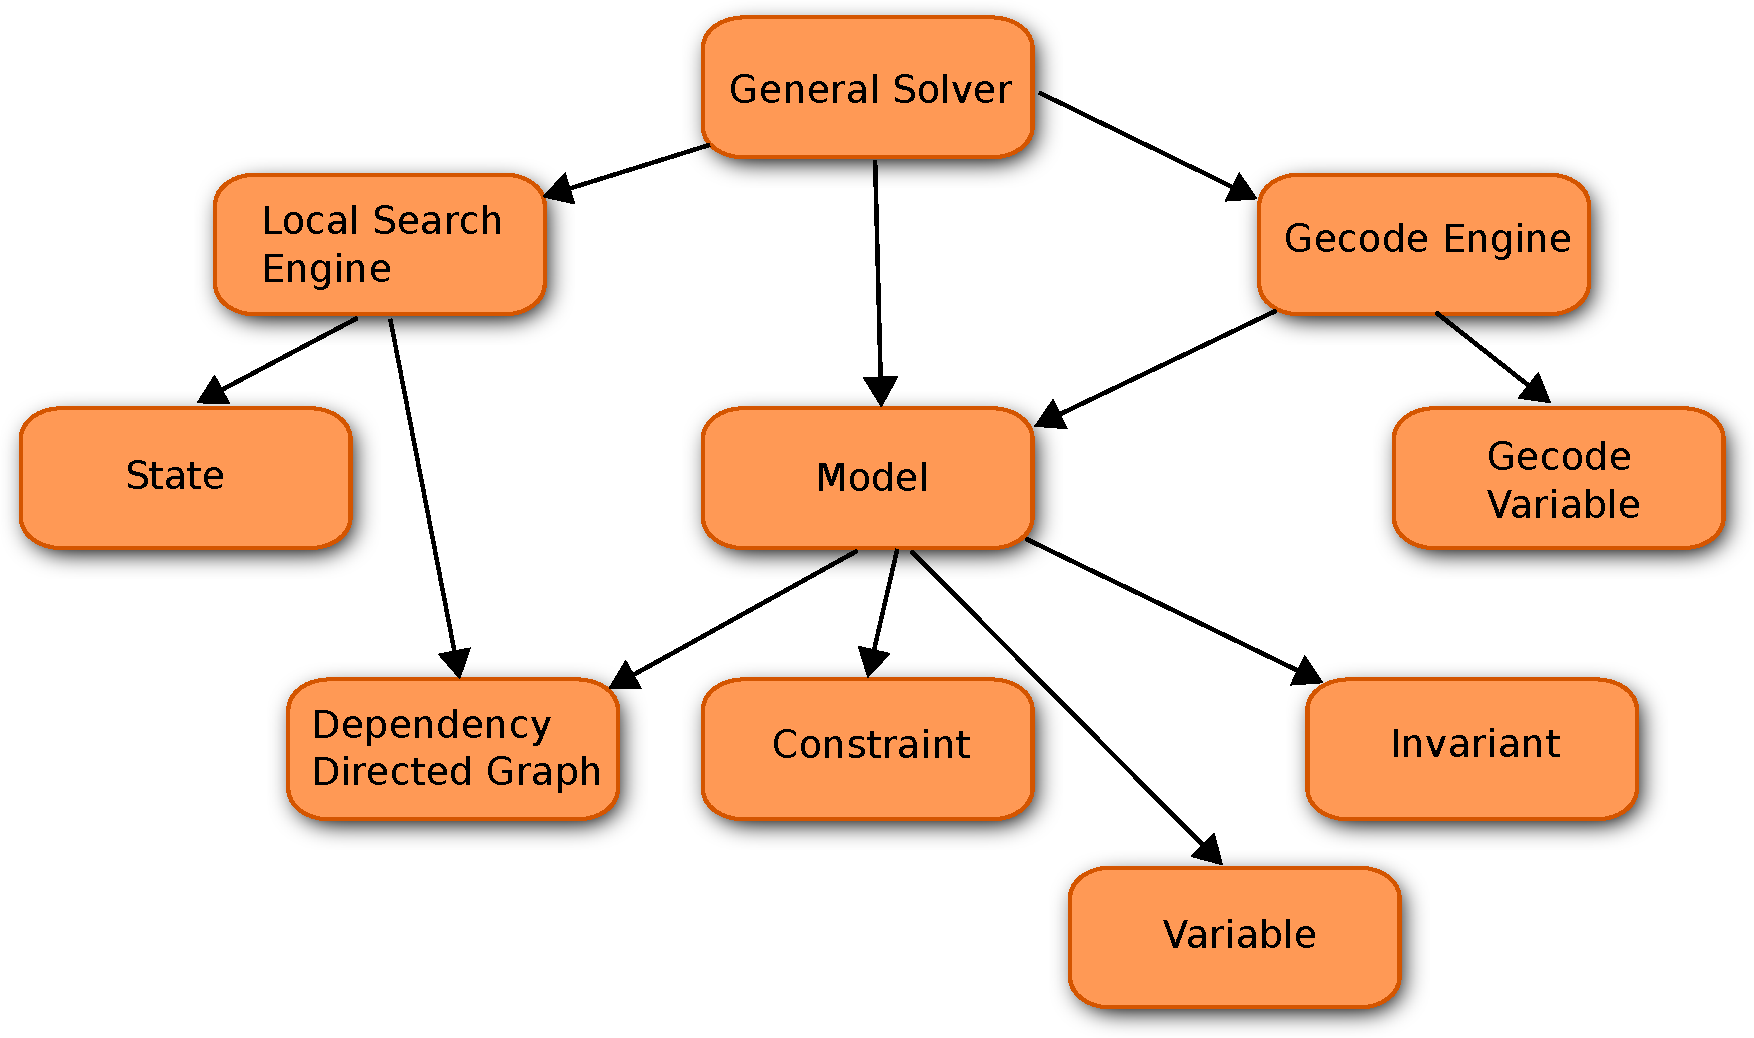
\includegraphics[width=\linewidth]{architectureTest}\caption{Overview of what the classes contains pointers to} 
\label{fig_architec}
\end{figure}
The main part of the solver is the \gensol class that functions like a distribution center, distributing tasks given 
by the user to the right part of the solver. The \gensol class contains 
the methods public to the user, such as creating variables and constraints, finding initial solution and optimizing the 
solution. \\ 
The two engines for solving are the \gecodesol and \lssol that find the initial solution and optimize the solution 
respectively. \gecodesol is used for preprocessing and finding an initial solution if possible with the limits given. 
\boste{Either just timelimit or could be made visible to the user by an option class with node, fail, and time limit.}  
This part will be elaborated further in section \ref{sec_gecode}. \\
\lssol is responsible for the optmization part of the solver with the use of local search and metaheuristics. \lssol 
transform the model to a CBLS model before the local search can start. How this is done and why will be discussed in 
section \ref{sec_ls}. \\ 
The Model class contains all variable, constraints and invariants and is used and altered by the previous three 
classes. Constraint and Invariant are parents to all constraint and invariant classes respectively. The contain 
abstract methods that the child classes must specify. The variable class is the only other class public to the user. A 
variable contains both the variable used by Gecode but is also used for local search. 

  \subsection{Variables}
  \subsection{Constraints}
  \begin{figure}[!b]
\centering
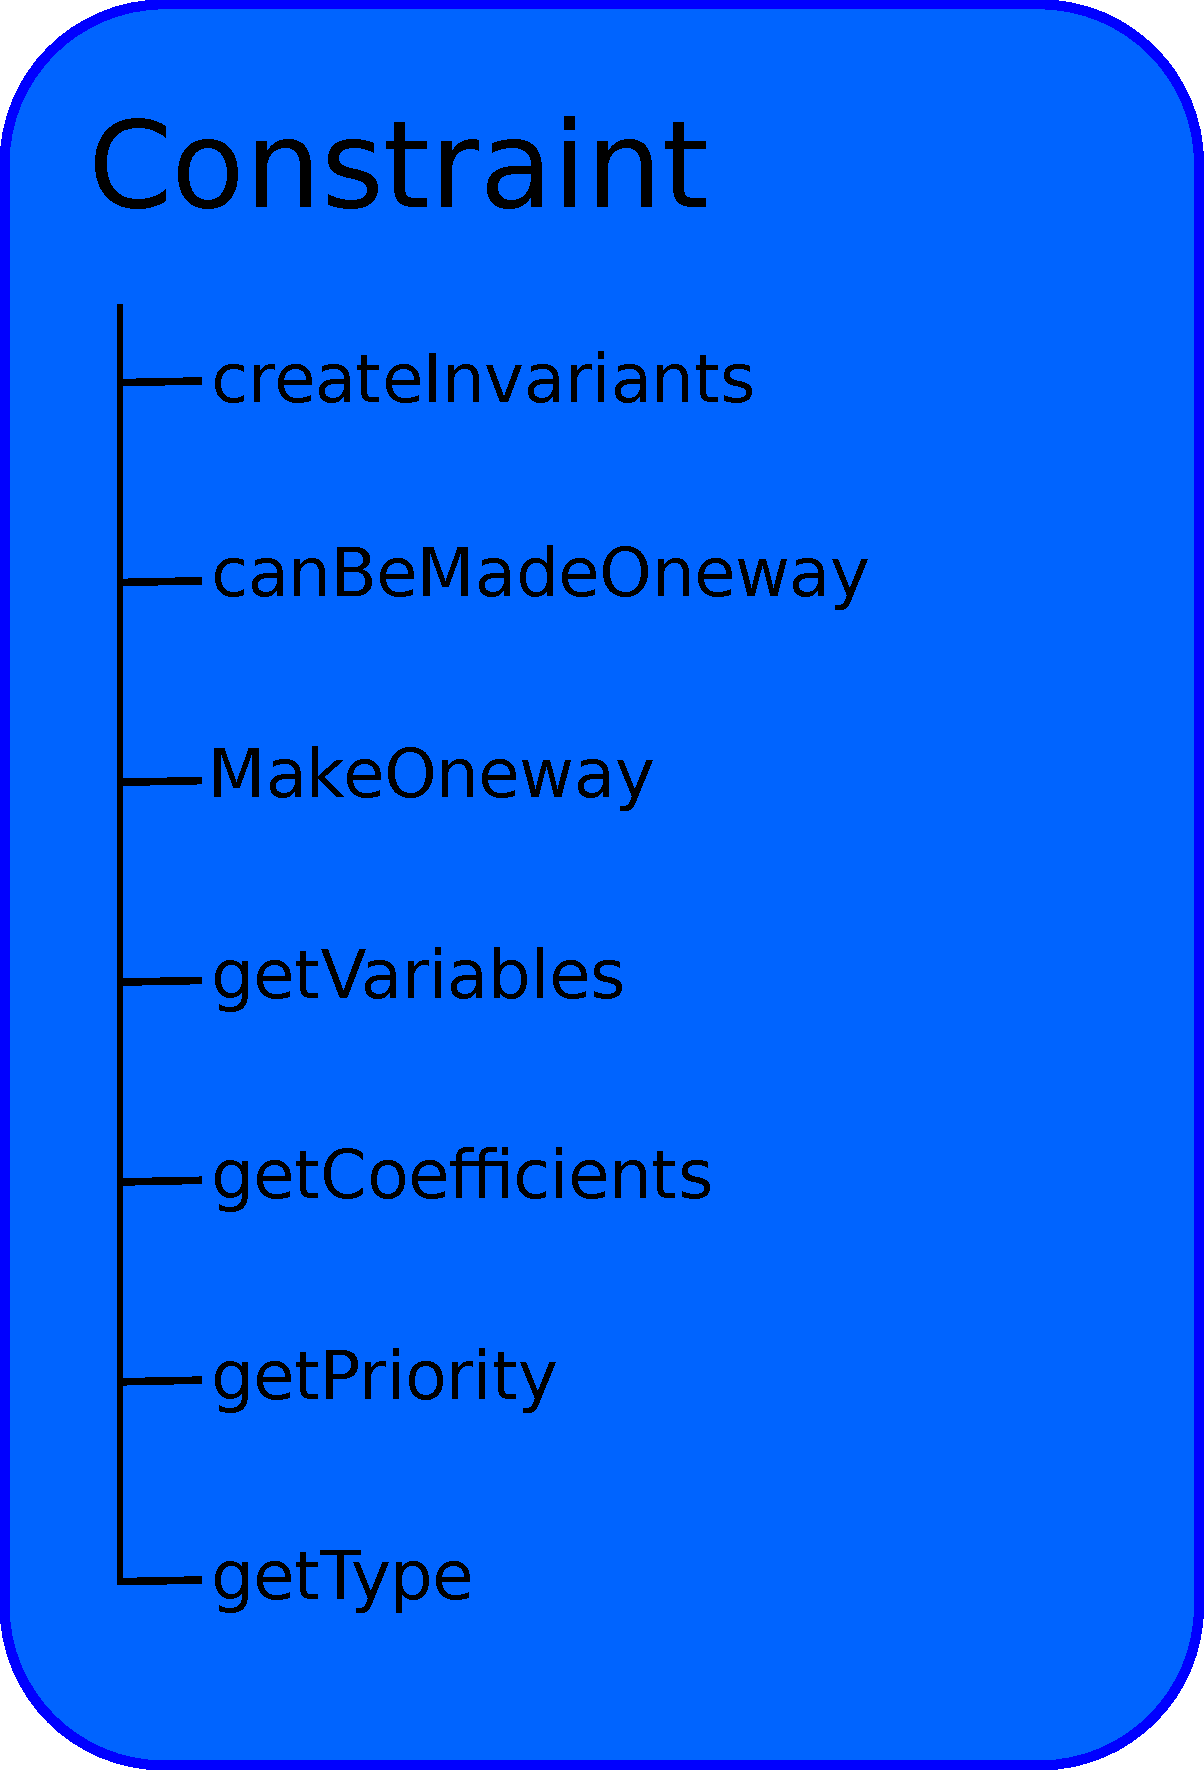
\includegraphics[width=\linewidth/2]{constraint.pdf} \caption{Important methods in Constraint 
class}\label{fig_constraint}
% \end{center} 
\end{figure}
Constraints are all derived from the same class (\class{Constraint} figure \ref{fig_constraint}) that forces some 
methods to be implemented. All constraints need a priority according to how important the constraint is. The priority 
is given by an positive integer and do not need to be unique but it will help the local search to differentiate between 
infeasible solutions. There is no reason to skip an integer in a sequence since it wont make a difference. It is 
suggested to keep the size of the sequence of priorities lower than 5. \\
An example of a constraint is the \class{Linear} constraint, which is the same as the one used in integer and binary 
programming, equation \ref{equat_linear} is an example of a \class{Linear} constraint. 
\begin{equation}
 c_1: \; 2x_1 + 2x_2 \leq 2  \qquad x_1,x_2 \in \{0,1\}
\end{equation} \label{equat_linear} \noindent
A constraint is posted in the Gecode \class{Space} by \class{GecodeEngine} and later handled in the 
\class{LocalSearchEngine}. The 
constraints are treated differently in the environments and need different parameters and methods for that. The LS 
environment handles constraints through invariants hence an implementation of a constraint needs a method for 
creating the invariants needed in LS. The method \method{createInvariants} creates invariants that 
might be auxiliary variables helpful during local search and one invariant that represents 
if the constraint is violated and the violation degree. The violation degree can be one if violated and zero 
otherwise, or it give a measurement of violated the constraint is. For the linear constraint $c_1$ in equation 
\ref{equat_linear} the violation degree is how much the value of the left hand side must decrease to satisfy the 
constraint. A helpful auxiliary variable is the value of the left hand side such that it does not need to be recomputed 
when computing the violation. \\
The methods \method{canBeMadeOneway} and \method{makeOneway} are used if the constraint can be transformed 
to a oneway constraint hence functionally define one of the variables. Method \method{canBeMadeOneway} returns a 
boolean whether it can be used or not and \method{makeOneway} transforms the constriant into a oneway constraint, 
implemented as an invariant, that defines one of the variables. The only constraint that has been implemented is 
\class{Linear}. 
\subsubsection{Implementation of Linear}
\class {Linear} is a linear constraint $c_j$ with a coefficient hashmap $A(c_j)$ and a vector of variables $X(c_j)$ 
that have some relation to a constant on the right hand side $b(c_j)$. The relation that can be used are: 
$\{\leq,=,\geq,>,<\}$ 
but only the first two ($\leq,=\}$) needs to be managed. If one of the three last is used it is transformed into a 
$\leq$ relation instead. This is done to reduce the number of comparisons later. The change can be done by multiplying 
with $-1$ on each side to change from ``greater'' to ``less'' relation. All coefficients and variables are integer hence 
all strictly less/greater relations can be transformed to a less/greater equal relation by increasing or decreasing 
$b(c_j)$ by 1. \\
The methods \method{canBeMadeOneway} and \method{makeOneway} are covered in section \ref{sec_ls} and only 
\class{Linear} constraints that have ``$=$'' relation can be made oneway constraints. \\ 
The method \method{createInvariants} creates two invariants the first one represents the value of the left hand side in 
the constraint and the other represents the violation degree. The first invariant is a \class{Sum} invariant and is 
described in the next subsection. The second one depends on the relation of the constraint and is either a 
\class{LEQVioaltion} or 
\class{EQVioaltion} that are also describe in the next subsection. \\
For notation if a variable is defined by an invariant it belongs to the set $Y(c_j)$ instead of $X(c_j)$. Algorithm 
\ref{algo_lin} illustrates how the two invariants for \class{Linear} is created. \\
\IncMargin{1em}
\begin{algorithm}[H]

%\SetKwFunction{relation}{relation}\SetKwFunction{coeff}{coefficient}
  \algdata
\Input{\cons $c_j$}
\Output{two invariants}
\BlankLine
	set invars $= \emptyset$\;
%         set coef = getCoefficients() \;
        \class{Sum} y = Sum($A(c_j)$,$X(c_j)$,$Y(c_j)$)\;
         \int value = sumInvariant.setValue()\;
         invars.add(sumInvariant)\;
         \If{getPriority() $\neq$ 0 } {
                \eIf{relation \upshape is '$\leq$'}{
                    LEQviolation leq = LEQviolation(sumInvariant, $b(c_j)$)\;
                     \eIf{value $\leq$ $b(c_j)$}{
                         $V(leq) =0$\;
                      }{
                          $V(leq) =(value - rightHandSide)$\;
                     }
                    invars.add(leq)\;
                } {
                   EQviolation eq = EQviolation(sumInvariant, $b(c_j)$)\;
                   \eIf{value == $b(c_j)$} {
                       $V(eq) =0$\;
                   }{
                       $V(eq) =|value - rightHandSide|$)\;
                   }
                   invars.add(eq)\;
                }
         }

        \Return invars\;
    
   
   
\caption{Linear - createInvariants()} \label{algo_lin} 
 %\caption{Test if a constraint $c$ can define a variable $x$ } \label{algo_checkoneway}
\end{algorithm} \noindent
\DecMargin{1em} \\


 \label{sub_cons}
  \subsection{Invariants}
  Invariants are all derived from one common class \class{Invariant}, see figure \ref{fig_invariant}, such that they 
all implements the same methods. This is very useful when doing local search. 
\begin{figure}[!b]
\begin{center}
 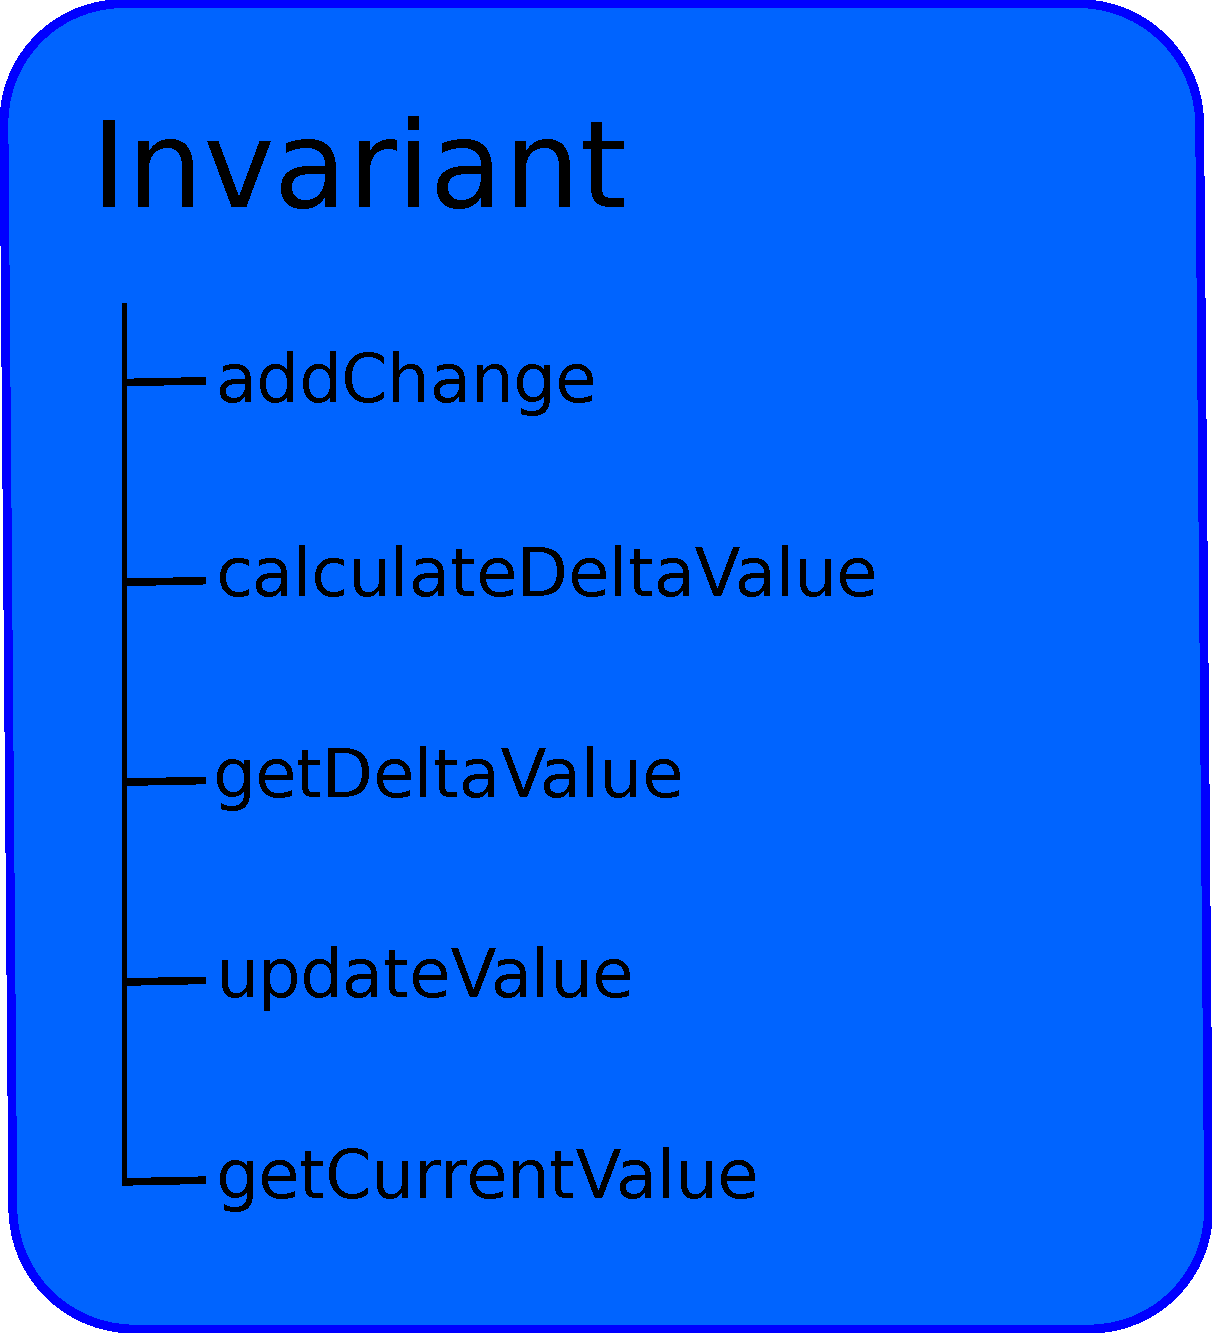
\includegraphics[width=\linewidth/2]{invariant.pdf} \caption{Important methods in Invariant 
class}\label{fig_invariant}
\end{center} 
\end{figure}
Invariants are only introduced after an initial solution to an instance has been found and before the local 
search has begun. Invariants can represent either a variable or an auxiliary variable and are defined by oneway 
constraints. The invariants classes that are implemented contain information about how the invariant is defined and the 
value of the invariant. Hence the \class{invariant} classes are representing both the oneway constraint and the 
invariant. \\ 
All subclasses of \class{Invariant} has a delta value, a current value, coefficient map, a stack of changes, a lower 
bound, and a upper bound. These are used by the different methods of the invariants. \\
All Invariants must implement the methods \method{proposeChange}, \method{calculateDelta}, and 
\method{updateValue} that are used during local search. When suggesting a new 
value to a variable the method \method{proposeChange} is used. The proposed change is put on the stack until the 
the method \method{calculateDelta} is called. \method{calculateDelta} is by the delta evaluation function in local 
search and updates the delta value of the invariant according to the changes received from \method{proposeChange}. The 
method \method{updateValue} is called when a neighborhood operation is commited, to update the value of the invariant. 
\\ Each type of invariant must implement its own method since the methods can be different for each type of invariant. 
\\ 
Different classes uses the invariants but do not differentiate between them since they all have the same methods.  
If invariants did not have a common super class then each invariant type would need its own data structure for 
storage. Another benefit is the search procedures do not have to examine which invariants the model consist of since 
they all have the same methods. It also makes it easier to add new invariants since all the functionality are 
implemented by the new invariant and nothing has to be changed in the \class{LocalSearchEngine}. \\ 
\subsubsection{Implementation of Sum}
The class \class{Sum} is used to define variables or auxiliary variables by a summation of variables multiplied by 
their coefficient with a constant offset. I.e. $x_1 = 2x_2+4x_3 + 1$, \class{Sum} can represent the right hand side in 
the equation defining $x_1$. \\ 
The method \method{proposeChange}(int  $variableID$, int $changeInValue$) uses the variables id to 
get its coefficient from a hashmap. The coefficient multiplied by the integer $changeInValue$, the change of the 
variables value, gives the delta value that is pushed on a stack $variableChange$. \\ 
The method \method{calculateDelta}() first reset the delta value to zero and then popping each integer on the stack 
and add them to the delta value. The implementation can be seen in algorithm \ref{algo_calcDelta}. 

\IncMargin{1em}
\begin{algorithm}[H]

%\SetKwFunction{relation}{relation}\SetKwFunction{coeff}{coefficient}
  \algdata
\Input{stack VariableChange}
\Output{\bool allowed}
%\BlankLine
    \int $DeltaValue$ = 0 \;
    \While{VariableChange $\neq \emptyset$}{
        $DeltaValue$ += VariableChange.pop()\;
    }
    \uIf{$DeltaValue + CurrentValue < lowerbound$} {
        \Return \false\;
    }\uElseIf{$DeltaValue + CurrentValue > upperbound$}{ 
  \Return \false \;
    }\Else{
    \Return \true \;
    }
\caption{Sum - calculateDelta()} \label{algo_calcDelta} 
 %\caption{Test if a constraint $c$ can define a variable $x$ } \label{algo_checkoneway}
\end{algorithm} \noindent
\DecMargin{1em} \\
It checks if the new value would violated the bounds of the \class{Invariant} in case it is used to define a variable. 
By returning false it tells the new value would not be within the bounds of the invariant hence the change cannot be 
allowed. This will 
be used during local search in section \ref{sec_local}. \\
It updates the by adding the delta value to the current value in the method \method{updateValue()}.

\subsubsection{Implementation of LEQViolation and EQViolation}
The invariant \class{LEQViolation} and \class{LEQViolation} are used for measuring violation of a constraint. They are
a relation between the value of an invariant and an integer. The value of \class{LEQViolation} is zero if and only if 
the value of the invariant is less than the integer. The value is the difference between the invariants value and the 
integer otherwise. For \class{LEQViolation} the value is zero if they are equal value otherwise the absolute value of 
the difference. \\ 
\method{proposeChange} and \method{updateValue} are implemented almost same as in \class{Sum} but 
\method{proposeChange} does not use the coefficient hashmap. \\ 
Algorithm \ref{algo_calcDelta2} and \ref{algo_calcDelta3} is the implementation of \method{calculateDelta}. \\ 
\IncMargin{1em}
\begin{algorithm}[H]

%\SetKwFunction{relation}{relation}\SetKwFunction{coeff}{coefficient}
  \algdata
\Input{stack VariableChange, \int LHS}
\Output{\bool allowed}
\BlankLine
    \If{VariableChange $= \emptyset$}{
      $DeltaValue$ = 0 \;
      \Return \true\;
    }
    \eIf{LHS + VariableChange.pop() $\leq$ RHS} {
    $DeltaValue = -CurrentValue $\;
    }{
      \int $old = max(LHS-RHS,0) $\;
      \int $new = max(LHS+VariableChange.pop() - RHS,0) $\;
      $DelataValue = new-old $\;
    }
    \Return \true \;
\caption{LEQViolation - calculateDelta()} \label{algo_calcDelta2} 
 %\caption{Test if a constraint $c$ can define a variable $x$ } \label{algo_checkoneway}
\end{algorithm} \noindent
\DecMargin{1em} \\

\IncMargin{1em}
\begin{algorithm}[H]

%\SetKwFunction{relation}{relation}\SetKwFunction{coeff}{coefficient}
  \algdata
\Input{stack VariableChange, \int LHS}
\Output{\bool allowed}
\BlankLine
    \If{VariableChange $= \emptyset$}{
      $DeltaValue$ = 0 \;
      \Return \true\;
    }
    \eIf{LHS + VariableChange.pop() $\leq$ RHS} {
    $DeltaValue = -CurrentValue $\;
    }{
      \int $old = max(LHS-RHS,0) $\;
      \int $new = max(LHS+VariableChange.pop() - RHS,0) $\;
      $DelataValue = new-old $\;
    }
    \Return \true \;
\caption{EQViolation - calculateDelta()} \label{algo_calcDelta3} 
 %\caption{Test if a constraint $c$ can define a variable $x$ } \label{algo_checkoneway}
\end{algorithm} \noindent
\DecMargin{1em} 
The bounds of these invariants are always satisfied. 

\label{sub_inv}
  \subsection{General Solver}
  The \gensol class contains the most high level methods and most of them are used directly by the user. An overview of 
the most important methods is shown in figure \ref{fig_general}. \\ \noindent
\begin{figure}[!b] 
\begin{center}
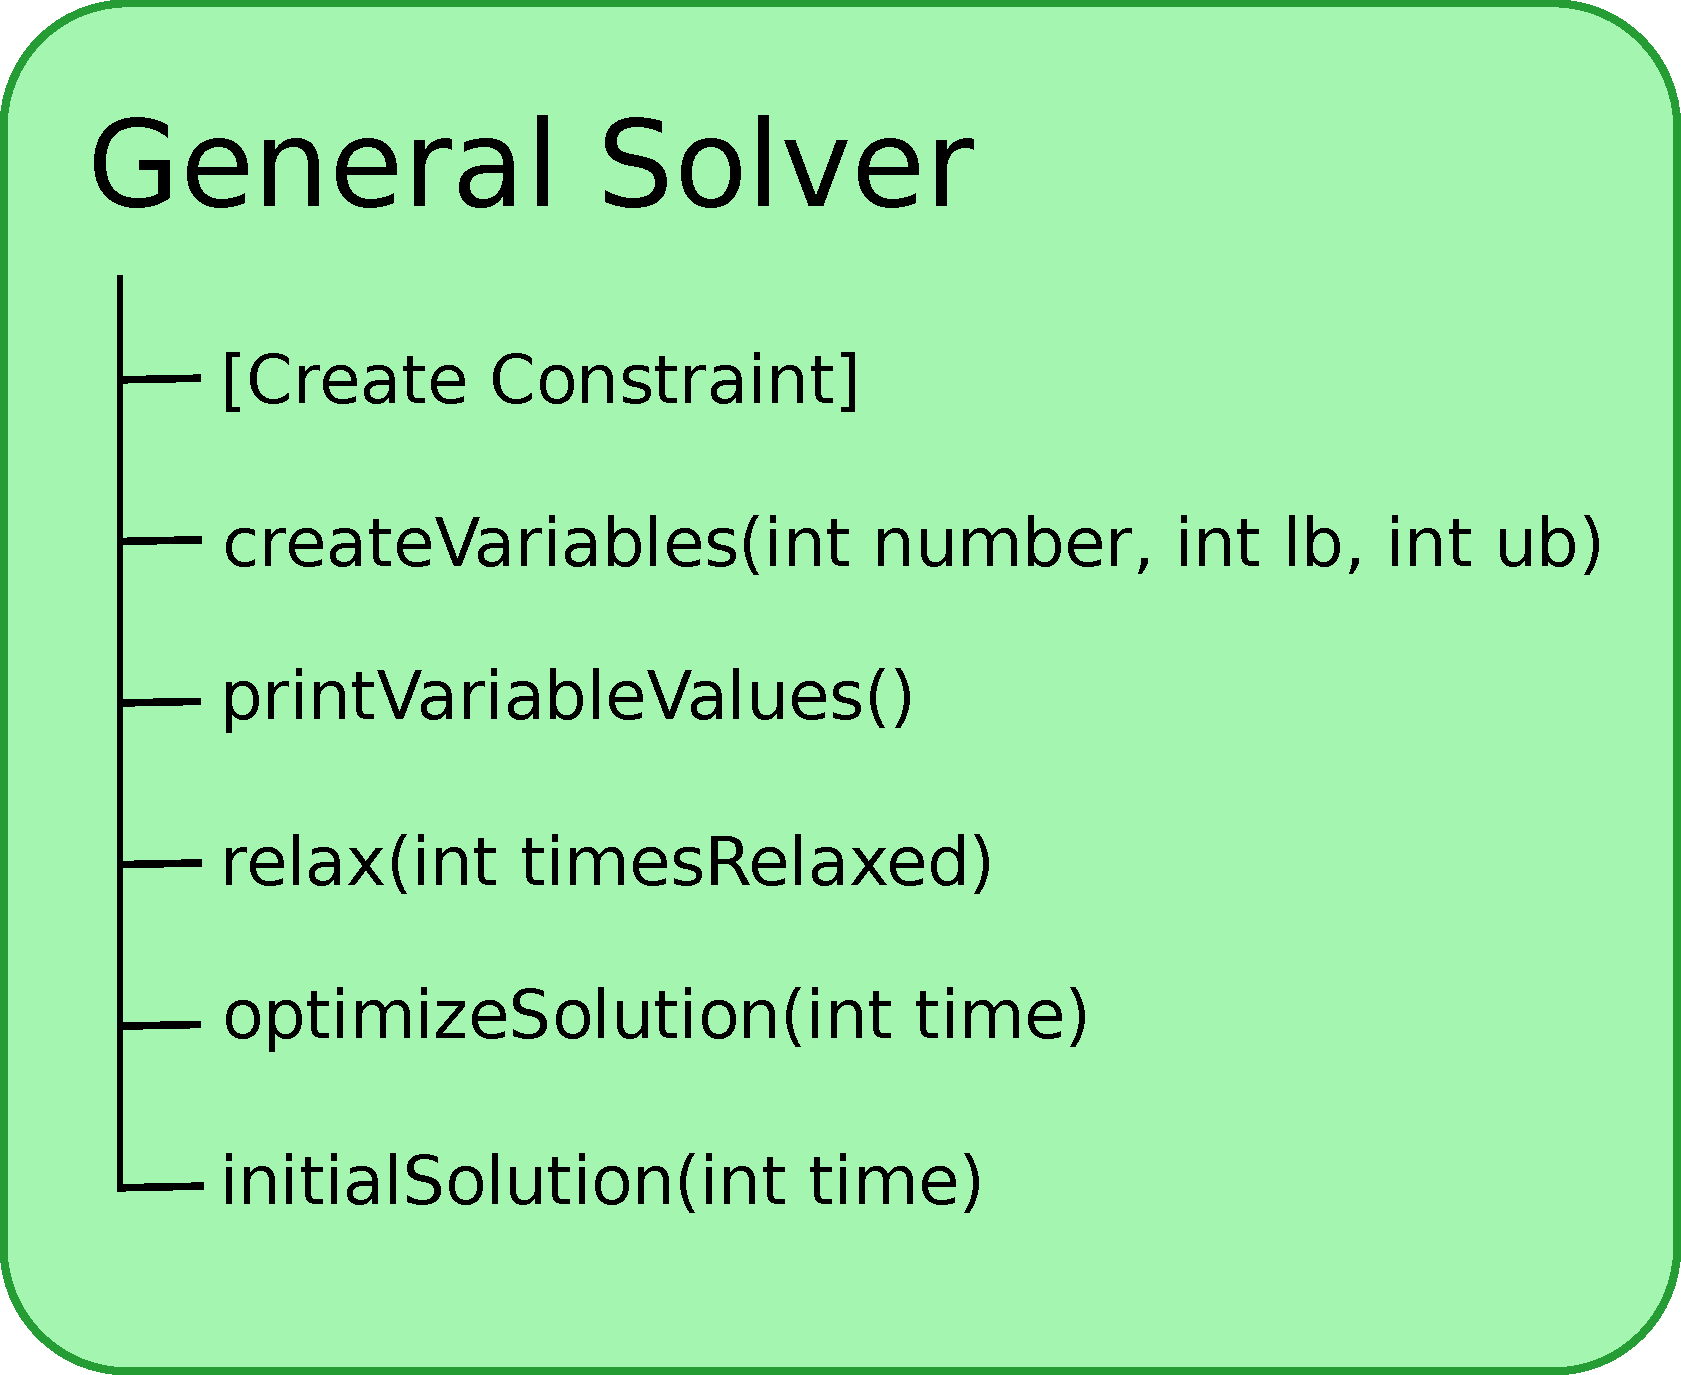
\includegraphics[width=0.8\linewidth]{general2.pdf} \caption{Important methods in GPSolver class} 
\label{fig_general}
\end{center} 
\end{figure} 
The method \method{createVariables} takes three arguments to create a number of variables. The first argument 
is the number of variables to create with the given lower and upper bound, the second and third argument respectively. 
The method creates both the gecode variables used in the \class{GecodeEngine} and variables used in the 
\class{LocalSearchEngine} class. The variables used in the \class{LocalSearchEngine} class (LS variables) are of the 
class 
\class{Variable} and each has a pointer to the associated Gecode variable. The method returns pointers to the LS 
variables. \\ 
The method \method{relax} is only used if an initial solution could not be found within the limits given. It controls 
how the instance should be relaxed to find an initial solution. There is currently only one method implemented that 
relaxes the an instance that is described in subsection \ref{sub_inisol}. \\
All constraint available are created by calling the associated method in \gensol, that calls the constructor 
of the constraint and the method in \class{GecodeEngine} for posting the constraint in a Gecode space. The constraint 
objects should not be created directly by the user since the Gecode \class{Space} class is not available to the 
user. \\ 
To implements a new constraint object it must inheriting from the \class{Constraint} class 
and two methods, one in \class{GPSolver} and one in \class{GecodeEngine}, must be implemented. The method in 
\class{GecodeEngine} must post the constraint in the \class{GecodeEngine} space. The method in \class{GPSolver} 
should call the constructor of the constraint implemented and call the method in \class{GecodeEngine}. The solver must 
be able to reproduce the call to \class{GecodeEngine} in case it an initial solution is not found within the limits 
given. The relaxation method must be updated to handle the new constraint implemented as well. \\
To find an initial solution the method \method{initialSolution} must be called and it takes an integer argument. The 
argument indicates the time Gecode is allowed to search for an initial solution before \method{relax} is called. Once 
\method{relax} is called the same time limit is given again. \\
To find a better solution than the initial solution the method \method{optimizeSolution} can be called with a time 
limit as argument. That method starts the local search that is described in section \ref{sec_local}. \label{sub_gen}
  
\newpage
\section{Preprocessing and Initial Solution} \label{sec_gecode}
  Each time a constraint is posted by a user it is parsed from General Solver to the Gecode Solver. The Gecode solver is 
derived from Gecode Space \boste{Define structure / Space before this} and the constraints parsed is posted in the 
Gecode Solver. Gecode has a large selection of constraints that can be used \cite[p. 58-80]{MPG:M}. Most of the 
constructors of these constraints are overloaded such that they can take different arguments and works with different 
types of variables. 
  \subsection{Domain Reduction}
  When an initial solution to the model is requested, Gecode \method{Branch()} method is called that specifies which 
variables to branch on and what values should be examined in the branches. Gecode uses preprocessing before searching 
for a solution and that might reduce the domain of some of the variables. If the domain of a variable is reduced to a 
single value, the variable is said to be fixed and is assigned that value. The variable will never change value hence 
it is no longer considered an independent variable.   
  \subsection{Finding an Initial Solution}
  Once domain reduction preprocessing has been done a Gecode DFS search engine (Depth First Search) is started. The stop 
criteria for Gecodes search can be specified by an option class. A Gecode search engine takes a space and search 
option as arguments and the search option contains a stop object. The stop object can either be timestop, nodestop or 
failstop. Each time Gecode branches on a variable two new nodes are created and nodestop set a upper bound on the 
number of nodes to explorer. If Gecode reaches a node that has no feasible assignment of one or more variables then 
that space is failed and failstop sets an upper bound on the number of failed spaces that can occur before stopping. 
Timestop stops the search if the time limit is reach. \\ 
Instead of using only one of these stop objects, a \class{Multistop} object has been implemented that combines all 
three stop objects such that it can have multiple stopping criterion. \\ 
Combinatorial problems can be formulated with Gecode and these problems can be very difficult to solve. In these cases 
Gecode keeps searching for a solution until it finds one (or runs out of available memory). Instead, the search can be 
stopped using stop object and the constraints can be relaxed such that Gecode can find a initial solution to the 
instance. If one of the stop criteria is reached the \method{relax} is called and some of the constraint are relaxed. To 
relax some constraints a new \class{GecodeEngine} is created and all variables and constraints, except those relaxed, 
are created and added to the new space. In order to choose which constraint that should be removed the priority of the 
constraints, given by the user, is used. The constraint is only relaxed if all non functional constraints with lower 
priority has been relaxed. The functional constraints are the last to be relaxed no matter what their priority are. The 
reason for this choice is these constraints are used to create oneway constraints and are only created if the 
functional constraints are feasible. \\
The constraints are chosen by their priority and ties are broken at random. I.e. a model with 100 
non-functional constraints of 
priority 3, 40 of priority 2, and 15 of priority 1 and there are 20 constraints that should be relaxed. The 15 
constraints with priority 1 and 5 of the 40 constraints with priority 2, chosen at random, would not be posted. The 
constraints that are not posted in the Gecode space are still applied when doing local search, hence the initial 
solution might start with some violations.  \\
A greedy approach is chosen in order to keep the time usage low. Each time Gecode fails in finding a solution the number 
of constraints added next time is halved. This is repeated at most 2 times, down to posting 25 \% of the constraints. If 
no solution can be found within the search 
limits, the search is stopped and finding an initial solution to the instance with Gecode has failed.  \\
If Gecode fails to find an initial solution, the independent variables are assigned value within their domain chosen 
uniformly at random.  \label{sub_inisol}

\newpage
\section{Structuring Local Search Model} \label{sec_ls}
Once an initial solution to the constraint satisfaction problem (CSP) has been found by Gecode the model is transformed 
to create a model better suited for local search, a CBLS model. Two new structures \boste{concepts, objects? Not sure 
what to call them} are introduced in this section, dependency directed graph \boste{directed dependency graph?} in 
subsection \ref{sec_ddg} and propagation queue in subsection \ref{sec_propaqueue}.  The dependency directed graph is 
used to update invariants dependent when a variable or invariant changes value. A propagation queue $q_i$ is created 
for each variable $x_i$ and it gives an ordering of the invariants directly or indirectly dependent on $x_i$. \\
%When a variable $x$ changes value other variables dependent on the value of $x$ will need to be updated. To 
%update those variables and invariants a directed graph $G=(V,A)$ is made, called dependency directed graph, 
%\emph{DDG}. 
%The vertices $V$ either represent a variable, an invariant or a constraint. \\  
%When one or more variables change value they propagate their change to the invariants pointed in $G$ that might point 
%to other invariants and propagate their changes to them. We only want to visit each vertex in the graph $G$ at most 
%one 
%time when making changes to on or more variables to increase performance. For each variable used in 
%the local search a \emph{propagation queue} $q$ is made. A propagation queue is the order of which invariant to update 
%when the associated variable changes value. \boste{Not quite happy about the description here} \medskip \\
The following changes to the model are made before the local search can begin. 
\begin{itemize}
 \item Define integer variables by oneway constraints
 \item Define binary variables by oneway constraints 
 \item Create auxiliary invariants for the remaining constraints
 \item Create a dependency directed graph
 \item Create propagation queue for all non-fixed and non-defined variables
%\item Initialize the invariants
% \item Initialize the constraints
% \item Initialize the objective function
\end{itemize}
When a variable is defined by a oneway constraint it is transformed into an invariant since its value is dependent on 
other variables and invariants. 
  \subsection{Simplification}
  The idea is to reduce the number of independent variables reducing the search space and likely the neighborhoods in 
local search. This does come with a downside that calculation of a variable changing value might take more time. \\ 
The functional constraint used to create a oneway constraint must be satisfied by the initial solution in order to 
create a oneway constraint. Once a oneway constraint is made it defines a variable that is represented by an invariant. 
The invariants value is always within the domain of the variable which corresponds to the functional constraint always 
being satisfied. \\
Even though all \class{Linear} constraints with an equality relation are functional only those with unit 
coefficients are chosen to be functional for simplicity. I.e. on the form $c: \sum\limits_{i=1}^{\alpha(c)} a_i 
x_i = b(c), \; |a_i|= 1 \; \; \forall i $. If other coefficients where allowed it could create non integer coefficients 
that does not work with the rest of the framework currently. \boste{Sikkert et spørgsmål til forsvar} \\ 
For each functional \class{Linear} constraint $c_j$ with unit coefficient two algorithm steps are used to create 
invariants. The first checks if the constraint $c_j$ can be transformed into a oneway constraint and the other 
transforms $c_j$ into a one-way constraint defining $x_i$. \\ 
\IncMargin{1em}
\begin{algorithm}[H]

%\SetKwFunction{relation}{relation}\SetKwFunction{coeff}{coefficient}
\SetKwFunction{makeOneway}{makeOneway}
\SetKwFunction{defi}{defines}
\algdata
 \Input{\cons $c_j$}
%\Output{Boolean}
\BlankLine
%\If{c \upshape already defines a oneway constraint}{\Return{} \false\; \boste{This constraint could be removed in 
%$O(\alpha(c_j))$}}
% \If{\upshape Number of integer variables not defined $> 1$}{\Return{} \false\; \boste{Needed in order to create the 
% right update queue}}
%\If{$|Y(c)| > 1$}{\Return{} \false}
%\If{\relation{c} \upshape is (==) }{\Return{} \true}
%\If{$c_j$ \upshape is not a linear equality}{
%  \Return{} \false}
%\int coeff = \coeff{c,v}\;
%\upshape in $\bigcup\limits_{o \in O} f_o(\vec{v})$}{	
%\tcp{Find the best variable to define}
\var $bestVariable$ = NULL\;
\int numberOfTies = 0 \;
 \ForEach{$x_i$ \upshape in $X(c_j)$ }{
%   \If{$x_i$ \upshape is fixed or defined}{
%     \continue
%   }
  \tcp{Break ties}
 % bestVariable = \decideBest{$x_i$,bestVariable} \;
  \If{\defi{$x_i$} $<$ \defi{$bestVariable$}}{
  \tcp{Choose the variable that helps define fewest invariants}
    $bestVariable$ = $x_i$ \;
    numberOfTies = 0 \;
%    \continue
  }
   \ElseIf{\defi{$x_i$} $==$ \defi{$bestVariable$}}{  
%     \If{$|D(x_i)|$ $>$ $|D(bestVariable)|$}{
%       \tcp{Choose the variable with largest domain size}
%       $bestVariable$ = $x_i$ \;
%       numberOfTies = 0 \;
%  %     \continue
%     } 
%     \ElseIf{$|D(x_i)|$ $==$ $|D(bestVariable)|$}{  
      \If{$|deg(x_i)|$ $<$ $|deg(bestVariable)|$}{
	\tcp{Choose the variable with lowest degree} \;
	$bestVariable$ = $x_i$ \;
	numberOfTies = 0 \;
%	\continue
      } 
      \ElseIf{$|deg(x_i)|$ $==$ $|deg(bestVariable)|$}{
	\tcp{Fair random} %\boste{Should this be further explained? (after alg)} 
	numberOfTies++ \;
	\If{Random(0,numberOfTies) == 0}{
	  $bestVariable$ = $x_i$ \;
	}
      }
%     }
   }
}

\If{ bestVariable $\neq $ \upshape NULL}{
  \makeOneway{\Var bestVariable} \;
 % \Return{} \true
}

%\Return{} \false \;
%\Return{} \true\;

\caption{Linear - canBeMadeOneway()} \label{algo_checkoneway} 
% \caption{Test if a constraint $c$ can define a variable $x$ } \label{algo_checkoneway}
\end{algorithm} \noindent
\DecMargin{1em} \\
For each unit \class{Linear} constraint an independent variable is found if possible. If there is more 
than one eligible variable the best variable among those is found. The first tiebreaker is the number of oneway 
constraints the variable participate in (helps define other variables). The next tiebreaker is the number of constraints 
the variables participate in. If none of the tiebreakers can be used a fair random is used such that the probability is 
equal for all variables whose ties could not be broken. \\ 
Once a the best variable is found, if any, algorithm \ref{algo_makeoneway} \makeOneway is called. \\
%\begin{itemize}
% \item Highest search priority or highest domain size
% \item Lowest size of $C(x_i)$
% \item Fair random 
%\end{itemize}
%The variables that a constraint $c$ applies to is the scope $V(c)$. The constraints are of the type \class{Linear} and 
%a constraint $c$ have a right hand side $B(c)$. \\
\IncMargin{1em}
\begin{algorithm}[H]
\algdata
\Input{\Var $x_i$, \cons $c_j$}
\Output{A new invariant $y$ defined by a oneway constraint}
\BlankLine
set $Q = \emptyset$ \tcp*[r]{new coefficient set}
set $U = \emptyset$ \tcp*[r]{new variable set}
\tcp{Move other variables to right hand side and update their cofficient}
\ForEach{$x_k$ \upshape in $X(c_j)\setminus {x_i}$}{
  $c'_{kj} = -\frac{c_{kj}}{c_{ij}}$ \;   
  $Q = Q\cup c'_{kj}$ \;
  $U = Q\cup x_k$ \;
}
\tcp{Isolate $x_i$ }
\int $b' = \frac{b(c_j)}{c_{ij}}$ \; 
\textbf{invariant} $y = $ \Sum($U$,$Q$,$b'$)\; \tcp{Invariant whose value is defined by the other variables and a 
constant}
%$G$ = $G \cup \{inv\}$\; 
%$G$ = $G \setminus \{c_j\}$\; 
%$G$ = $G \setminus \{x_i\}$\;
  %\boste{Maybe remove $c$ from $G$}
  %\Return{\Sum{$V(c)$,$A(c)$,b}}

%\int $coef = A_{c,x}$\;
%$Q = A_c \backslash \{A_{c,x}\}$\;
%$U = V(c) \backslash \{x\}$\;
%\ForEach{$A_{c,x}$ \upshape in $Q$}{
%  $Q_{c,x} = A(c,x) \cdot \frac{-1}{coef}$
%}
%\int $b = B(c)$ \;
%\If{relation{c} \upshape is (==) }{
%  Invariant $c' = $ \Sum{$U$,$Q$,b}\;
%  $G$ = $G \cup c'$\; 
%  \boste{Maybe remove $c$ from $G$}
%  %\Return{\Sum{$V(c)$,$A(c)$,b}}
%}
%\Else{
%  Invariant $c' = $ \Sum{$U$,$Q$,b}\;
%  Invariant $c'' = $ \Max{c',lb(x)}\;
%  $G$ = $G \cup c'$\; 
%  $G$ = $G \cup c''$\; 
%  \boste{Maybe remove $c$ from $G$}
%  %\Return{\Max{inv,b}}
%}
 \caption{Linear - makeOneway(\textsf{Variable} $x_i$)} \label{algo_makeoneway}
\end{algorithm}\DecMargin{1em} \noindent
The algorithm transforms the constraint $c_j$ into a oneway constraint defining an invariant. The dependency directed 
graph $G$ is updated by adding the new invariant $y$ and removing the constraint $c_j$ and variable $x_i$. \medskip 
\\
The value of the invariant must always be within its domain, corresponding to domain of the variable. It is not allowed 
to change value of one of the variable such that the invariants value is not within its domain.
%\IncMargin{1em}
%\begin{algorithm}[H]
%\SetKwData{Oneway}{oneway}
%\SetKwFunction{makeOneway}{makeOneway}
%\SetKwFunction{Next}{next}\SetKwFunction{Constraints}{Constraints}\SetKwFunction{Remove}{remove}
%\SetKwFunction{canBeMadeOneway}{canBeMadeOneway}
%\algdata 
%\Input{A set $C$ of functional constraints sorted by increasing arity}
%\Output{A model better suited for local search}
%\BlankLine
%%\emph{special treatment of the first line}\;
%\Bool $change = $ \true\;
%\While{$C \neq \emptyset$ \textbf{and} $change$}{
%  $change = $\false \;
%  %\ForEach{$x \in X$}{
%  %  \upshape select \Var $x$ \upshape from $X$\;
%    \ForEach{\Con $c$ \upshape in $C$}{
%      \Bool $flag = $ \canBeMadeOneway{c}\;  
%      \If{$flag$}{
%	\makeOneway{c,x}\;
%	Remove $x$ from $X$\;
%	$change = \true$\;
%	\bre\;
%      }
%    }
%  }
%}
%\caption{Defining integer variables by one-way constraints}\label{makefunc}
%\end{algorithm}\DecMargin{1em}
%\noindent
%The following Two algorithms checks if the \cons $c$ can be transformed into a oneway constraint 
%and transforms $c_j$ into a one-way constraint defining $x$. 



%The algorithm creates invariants that defines variables $x_i \in X$ by one-way constraints. It uses two other 
%algorithms \canBeMadeOneway{$c_j$} and \makeOneway{$c_j$,$x_i$}. The first algorithm \\ 
%The complexity of algorithm \ref{algo_defintvar} depends on the complexity of the two other algorithms but for 
%simplicity let us assume they do not contribute for now. \\ 
%Let $\alpha_{max}$ be the largest arity among all constraints in $C$ and $n$ be the number of decision variables in 
%the 
%input set. The size of $X$ has decrease by at least one each time we pass line 3 except for the first time. Hence line 
%3 
%is passed at most $n$ times. Then the complexity of algorithm \ref{algo_defintvar} is $O(\alpha_{max} n^2)$. \\ 
%\medskip
%The coefficient of a variable $x_i$ in constraint $c_j$ is denoted $a_{ij}$. Let $\mathcal{F} = \{f_1,f_2,\dots 
%,f_k\}$ 
%be the family of objective functions \boste{Think we should discuss this Tuesday} and the coefficient of variable 
%$x_j$ in $f_k$ be $a_{kj}$. \boste{Maybe call it 
%evaluation functions. Does not make sense since $a_{34}$ refers both to constraint and obj. func} \\  



  \subsection{Dependency Digraph}
    \boste{What is the DDG? } \\ 
\boste{Why do we want a DDG?} \\
\boste{What properties should it have and why?} \\
The vertices $V$ in the dependecy directed graph (DDG) $G=(V,A)$ initially only represent the variables and the 
constraints where the varible vertices only have outgoing arcs to the constraints they participate in. We want to 
change the CSOP model to a model more suited for local search, a CBLS model. The initial model wil be modified by 
introducing invariants defined by oneway constriants and vertices representing invarints will be added to the graph 
$G$.  \\
The graph can be illustrated with all the variable vertices to the left and all constraint vertices to the right. 
Then the invariants vertices will be added in the middel. \\  
The invariants represents variables that are defined by oneway constraints or they can represent 
auxiliary variables used in the local search.
From now on when talking about vertices in $G$ it refers to the variable, invariant or constraint it represents unless 
other stated. \\
%The variables are non-fixed and non-defined and only have outgoing arcs. 
The vertex $v \in V$ has an outgoing arc to vertex $u \in V$ if and only if the value of $u$ is directly dependent on 
the value of $v$.
%Variables and invariants has an outgoing arc to the invariants that 
%depends on their value. \\ 
The DDG is needed in order to evaluate and update values of variables and invariants during local search. Local search 
is only performed on the variables 



Let us consider the following example with three variables and a two constraint.
\begin{center}
\begin{tabular}{rlr}
$ c_1: $&$2x_1 + x_2 - x_3 $&$= 2$ \\
$ c_2: $&$x_2 + x_3 $&$\leq 1$ \\
\end{tabular} 
\end{center}
Initially $G$ would consist of the three variables $x_1$, $x_2$, and $x_3$ and the constraints $c_1$ and $c_2$. The 
variable $x_3$ could be defined as an invariant $i_1$ by transforming $c_1$ to a oneway constraint. Once a 
variable is defined by a oneway constraint it is removed from the graph. Since $c_1$ is transformed it is removed from 
the $G$ and replaced by invariant $i_1$ which has ingoing arcs from $x_1$ and $x_2$. 

\begin{center}
    \begin{tikzpicture}[scale=1]
        \vertex[label=$x_1$](x1) at (0,2) {};
        \vertex[label=$x_2$](x2) at (0,0) {};
        \vertex[label=$i_1$](i1) at (2,1) {};
        \vertex[label=$c_2$](c2) at (4,0) {};

    \tikzset{EdgeStyle/.style={->}}
        \Edge(x1)(i1)
        \Edge(x2)(i1)
        \Edge(x2)(c2)
        \Edge(i1)(c2)
        %\Edge(y1)(c3)
        %\Edge(y2)(c3)
    \end{tikzpicture}
\end{center}
Auxiliary variable can be useful to speed up local search and in this example we could create an auxiliary 
variable $a_1$ which value is the sum of the left hand side of $c_2$. The auxiliary variable $a_1$ will be represented 
by an invariant $i_2$ which will be added to $G$. The invariant $i_1$, representing $x_3$, and variable $x_2$ have 
an outgoing arc to $i_2$ and $i_2$ have an outgoing arc to $c_2$. 


\begin{center}
    \begin{tikzpicture}[scale=1]
        \vertex[label=$x_1$](x1) at (0,2) {};
        \vertex[label=$x_2$](x2) at (0,0) {};
        \vertex[label=$i_1$](i1) at (2,1) {};
        \vertex[label=$i_2$](i2) at (4,0) {};
        \vertex[label=$c_2$](c2) at (6,0) {};

    \tikzset{EdgeStyle/.style={->}}
        \Edge(x1)(i1)
        \Edge(x2)(i1)
        \Edge(x2)(i2)
        \Edge(i1)(i2)
        \Edge(i2)(c2)

    \end{tikzpicture}
\end{center}
\boste{Talk about updating $x_2$}

%\end{minipage}
 
\boste{start on algorithms}
The DDG $G$ is initially a bipartite graph where all the decision variables $X$ are vertices in one set and all the 
constraints $C$ are vertices in the other set. If constraint $c$ applies to a variable $x$ then there is an arc from 
the vertex representing $x$ to the vertex representing $c$. \\    
First all integer variables $Y$ in the CSOP $\mathbb{P}$ \boste{Should I call the models CSOP or just model?} get 
defined by oneway constraints by algorithm 
\ref{algo_makeints}. If some of the integer varibles cannot be defined \boste{Currently report fail and exit}. 
\\
\IncMargin{1em}
\begin{algorithm}[H]
\SetKwData{Oneway}{oneway}
\SetKwFunction{makeIntVarOneway}{makeIntVarOneway}
\SetKwFunction{Next}{next}\SetKwFunction{Constraints}{Constraints}\SetKwFunction{Remove}{remove}
\SetKwFunction{intVarCanBeMadeOneway}{intVarCanBeMadeOneway}
\algdata 
\Input{A set $Y$ of integer variables sorted by decreasing domain size}
\Output{A CBLS model for local search}
\BlankLine
%\emph{special treatment of the first line}\;
\Bool $change = $ \true\;
\While{$Y \neq \emptyset$ \textbf{and} $change$}{
  $change = $\false \;
  \ForEach{$y_i \in Y$}{
    \upshape select \Var $y_i$ \upshape from $Y$\;
    \ForEach{\Con $c_j$ \upshape in $C(y_i)$}{
      \If{\intVarCanBeMadeOneway{$y_i$,$c_j$}}{
	\makeIntVarOneway{$y_i$,$c_j$}\;
	Remove $y_i$ from $Y$\;
	isOneway($c_j$) = \true \;
	$change = \true$\;
	\bre\;
      }
    }
  } \label{false}
}
\caption{Defining integer variables by one-way constraints}\label{algo_makeints}
\end{algorithm}\DecMargin{1em}
\noindent
For each of the variables $y_i$ each of the constraints $c_j$ that applies to $y_i$ is checked if it can be made oneway 
to define $y_i$ until one is found or none can be found. This is done until there are no integer variables left or the 
remaining integer variables cannot be defined, when the boolean change is false after line \ref{false}. Algorithm 
\ref{algo_checkintoneway} checks if constraint $c_j$ can be made oneway to define $y_i$ and algorithm 
\ref{algo_makeintoneway} transforms $c_j$ into a oneway constraint defining $y_i$ and updates the DDG $G$. \\
Let $\mathcal{F} = \{f_1,f_2,\dots ,f_k\}$ be the family of objective functions. \\
\IncMargin{1em}
\begin{algorithm}[H]

\SetKwFunction{relation}{relation}\SetKwFunction{coeff}{coefficient}
\SetKwFunction{objcoeff}{objectiveCoefficients}
\algdata
\Input{\Var $y_i$ and \Con $c_j$}
\Output{Boolean}
\BlankLine
\If{$c_j$ \upshape already defines a oneway constraint}{\Return{} \false\; \boste{This constraint could be removed in 
$O(\alpha(c_j))$}}

int $undefinedIntVar = 0$ \;
\ForEach{\Var $x$ \upshape in $c_j$}{
  \If{x is undefined integer variable}{
    $undefinedIntVar++$\;
  }
}
\If{$undefinedIntVar > 1$ \label{undefined}}{\Return{} \false  \boste{Insures no cycle is created} \; 
\tcp {else only $y_i$ is undefined integer variable}} 
%\If{$|Y(c)| > 1$}{\Return{} \false}
%\If{\relation{c} \upshape is (==) }{\Return{} \true}
\If{$c_j$ \upshape is linear equality}{\Return{} \true}
%\int coeff = \coeff{c,v}\;
%\upshape in $\bigcup\limits_{o \in O} f_o(\vec{v})$}{	
%\boste{The following is not at all correct, we should discuss this Tuesday} \\
\If{\upshape coefficient $c_{ij} \geq 0 $ \label{positivecoef}}{ 
  \Return{} \false \; 
}
\ForEach{ $f_j$  in $\mathcal{F}$ }{
  \If{$f_ij < 0$ \label{objectivecoef}}{
    \Return{} \false \;
    \boste{Not sure of to define coefficients in objective functions. coefficient of variable i in constraint j could 
be $c_{ij}$ but $c_j$ is used for constraint and then all variable $y_i$ should be $y_i$}
  }
}
\Return{} \true\;
 \caption{intVarCanBeMadeOneway( \textsf{Variable} $y_i$, \textsf{Constraint} $c_j$)} \label{algo_checkintoneway}
% \caption{Test if a constraint $c$ can define a variable $x$ } \label{algo_checkoneway}
\end{algorithm}
\DecMargin{1em}
If constraint $c_j$ already defines another variable it cannot be used to define $y_i$. Line \ref{undefined} makes sure 
that integer variable $y_i$ is not defining another integer variable $y_k$. This limits the model and increases the 
complexity of algorithm \ref{algo_makeints} because of the addition of the initial while loop. The 
condition in line \ref{undefined} makes sure that no strongly connected component of size 2 or greater is created in 
$G$. \boste{This should be described why we dont want that and what a SCC is}. The lines \ref{positivecoef} and 
\ref{objectivecoef} returns false if the coefficient of $y_i$ in $c_j$ is positive or one of the coefficients in the 
objective functions is negative. If that is not the case the constraint $c_j$ can define variable $y_i$ since we 
restrict the lower bound of $y_i$ by the oneway constraint and want to minimize its value in the objective functions. 
This gives some other complications which will be described after algorithm \ref{algo_makeintoneway}. \\ 
\IncMargin{1em}
\begin{algorithm}[H]
\algdata
\Input{\Var $y_i$ and \Con $c_j$}
\Output{Updated $G$}
\BlankLine
%\int $coef = A_{c,x}$\;
set $Q$ \tcp*[r]{new coefficient set}
set $U$ \tcp*[r]{new variable set}
\tcp{Move $y_i$ to right hand side and set coefficient to 1}
\ForEach{$x_k$ \upshape in $X(c_j)\setminus {y_i}$}{
  $c'_{kj} = -\frac{c'_{kj}}{c_{ij}}$ \;   
  $Q = Q\cup c'_{kj}$ \;
  $U = Q\cup x_k$ \;
}
%$Q = A_c \backslash \{A_{c,x}\}$\;
%$U = X(c) \backslash \{y_i\}$\;
%\ForEach{$A_{c,x}$ \upshape in $Q$}{
%  $Q_{c,x} = A(c,x) \cdot \frac{-1}{coef}$
%}
\tcp{Move right hand side to left hand side and update coefficient}
double $b' = \frac{B(c_j)}{c_{ij}}$ \;
\boste{coefficients can now be doubles (non integer)} \;
\If{$c_j$ \upshape is linear equality}{
  \textbf{oneway} $c' = $ new oneway($U$,$Q$,$b'$)\;
  $G$ = $G \cup \{c'\}$\; 
  $G$ = $G \setminus \{c_j\}$\; 
  %\boste{Maybe remove $c$ from $G$}
  %\Return{\Sum{$V(c)$,$A(c)$,b}}
} \Else {
    \boste{Remember to say all constraints are either LQ or EQ} \;
    \textbf{oneway} $c' = $ new oneway($U$,$Q$,$b'$)\;
    Invariant $c'' = $ new \Max{$c'$,lowerbound($y_i$)}\;
    $G$ = $G \cup c'$\; 
    $G$ = $G \cup c''$\; 
    $G$ = $G \setminus \{c_j\}$\; 
% \boste{Maybe remove $c$ from $G$}
  %\Return{\Max{inv,b}}
}

 \caption{makeIntVarOneway(\textsf{Variable} $y_i$, \textsf{Constraint} $c_j$)} \label{algo_makeintoneway}
 %\caption{Make one-way constraint from $c$ defining variable $x$ } \label{algo_makeoneway}
 \end{algorithm}\DecMargin{1em}
If the constraint $c_j$ is a linear equality constraint a new oneway constraint $c'$ is made by isolating $y_i$ on 
the right side. Then $c'$ is added to $G$ and $c_j$ is removed from $G$. If $c_j$ is not a linear equality constraint 
then it is a linear constraint with an upper bound $B(c_j)$. Since $c_ij$, the coefficient of $y_i$ in $c_j$, is 
negative $y_i$ can be isolated on the right hand side so $y_i$ is the upper bound for the left hand side. The 
coefficients of $y_i$ in the objective functions are non-negative   


Once all integer variables 
have been defined by oneway constraints, algorithm \ref{makefunc} is used to make each functional constraint into a 
oneway constraint defining a binary variable if possible. \\ 





Let $X$ be a set of variables and $x \in X$. The subset of constraints $C(x) \subseteq C$ is the set 
of constraints that applies to $x$.\\ 
The following algorithms describe how one-way constraints a create to define a variable $x$. \\ 



\IncMargin{1em}
\begin{algorithm}[H]
\SetKwData{Oneway}{oneway}

\SetKwFunction{makeOneway}{makeOneway}
\SetKwFunction{Next}{next}\SetKwFunction{Constraints}{Constraints}\SetKwFunction{Remove}{remove}
\SetKwFunction{canBeMadeOneway}{canBeMadeOneway}
\algdata 
\Input{A set $X$ of variables \boste{Sorting order?}}
\Output{A model better suited for local search}
\BlankLine
%\emph{special treatment of the first line}\;
\Bool $change = $ \true\;
\While{$X \neq \emptyset$ \textbf{and} $change$}{
  $change = $\false \;
  \ForEach{$x \in X$}{
    \upshape select \Var $x$ \upshape from $X$\;
    \ForEach{\Con $c$ \upshape in $C(x)$}{
      \Bool $flag = $ \canBeMadeOneway{c,x}\;  
      \If{$flag$}{
	\makeOneway{c,x}\;
	Remove $x$ from $X$\;
	$change = \true$\;
	\bre\;
      }
    }
  }
}
\caption{Defining integer variables by one-way constraints}\label{makefunc}
\end{algorithm}\DecMargin{1em}
\noindent
The algorithm tries to create invariants that define the set of variables $X$ by one-way constraints. It uses two other 
algorithms \canBeMadeOneway{c,x} and \makeOneway{c,x}. The first algorithm checks if the \cons $c$ can be used to define 
\var $x$ and the second algorithm transforms $c$ into a one-way constraint defining $x$. \\ 
The complexity of algorithm \ref{algo_defintvar} depends on the complexity of the two other algorithms but for 
simplicity let us assume they do not contribute for now. \\ 
Let $\alpha_{max}$ be the largest arity among all constraints in $C$ and $n$ be the number of decision variables in the 
input set. The size of $X$ has decrease by at least one each time we pass line 3 except for the first time. Hence line 3 
is passed at most $n$ times. Then the complexity of algorithm \ref{algo_defintvar} is $O(\alpha_{max} n^2)$. \\ \medskip
The coefficient of a variable $x_j$ in constraint $c_i$ is denoted $a_{ij}$. Let $\mathcal{F} = \{f_1,f_2,\dots ,f_k\}$ 
be the family of objective functions \boste{Think we should discuss this Tuesday} and the coefficient of variable $x_j$ 
in $f_k$ be $a_{kj}$. \boste{Maybe call it 
evaluation functions. Does not make sense since $a_{34}$ refers both to constraint and obj. func} \\  

\IncMargin{1em}
\begin{algorithm}[H]

\SetKwFunction{relation}{relation}\SetKwFunction{coeff}{coefficient}
\SetKwFunction{objcoeff}{objectiveCoefficients}
\algdata
\Input{\Con $c$ and \Var $x$}
\Output{Boolean}
\BlankLine
\If{c \upshape already defines a oneway constraint}{\Return{} \false\; \boste{This constraint could be removed in 
$O(\alpha(c))$}}
\If{\upshape Number of integer variables not defined $> 1$}{\Return{} \false\; \boste{Needed in order to create the 
right update queue}}
%\If{$|Y(c)| > 1$}{\Return{} \false}
\If{\relation{c} \upshape is (==) }{\Return{} \true}
%\int coeff = \coeff{c,v}\;
%\upshape in $\bigcup\limits_{o \in O} f_o(\vec{v})$}{	
\boste{The following is not at all correct, we should discuss this Tuesday} \\
\ForEach{a \upshape in $A(f(x))$ }{
  \If{$A(c,x) \cdot a > 0$}{
    \Return{} \false
  }
}
\Return{} \true\;
 \caption{canBeMadeOneway(\textsf{Constraint} c, \textsf{Variable} x)} \label{algo_checkoneway}
% \caption{Test if a constraint $c$ can define a variable $x$ } \label{algo_checkoneway}
\end{algorithm}
\DecMargin{1em}
\boste{Description not finished (done at all)}

%The variables that a constraint $c$ applies to is the scope $V(c)$. The constraints are of the type \class{Linear} and 
%a constraint $c$ have a right hand side $B(c)$. \\ 
\IncMargin{1em}
\begin{algorithm}[H]
\algdata
\Input{\Con $c$ and \Var $x$}
\Output{An Invariant}
\BlankLine
\int $coef = A_{c,x}$\;
$Q = A_c \backslash \{A_{c,x}\}$\;
$U = V(c) \backslash \{x\}$\;
\ForEach{$A_{c,x}$ \upshape in $Q$}{
  $Q_{c,x} = A(c,x) \cdot \frac{-1}{coef}$
}
\int $b = B(c)$ \;
\If{\relation{c} \upshape is (==) }{
  Invariant $c' = $ \Sum{$U$,$Q$,b}\;
  $G$ = $G \cup c'$\; 
  \boste{Maybe remove $c$ from $G$}
  %\Return{\Sum{$V(c)$,$A(c)$,b}}
}
\Else{
  Invariant $c' = $ \Sum{$U$,$Q$,b}\;
  Invariant $c'' = $ \Max{c',lb(x)}\;
  $G$ = $G \cup c'$\; 
  $G$ = $G \cup c''$\; 
  \boste{Maybe remove $c$ from $G$}
  %\Return{\Max{inv,b}}
}

 \caption{makeOneway(\textsf{Constraint} c, \textsf{Variable} x)} \label{algo_makeoneway}
 %\caption{Make one-way constraint from $c$ defining variable $x$ } \label{algo_makeoneway}
 \end{algorithm}\DecMargin{1em}
\boste{Description of algorithm here} \\
Consider the following three constraints as a small example. \boste{Should the example be introduced before the 
algorithms?}
\begin{center}
\begin{tabular}{rlr}
$ c_1: $&$2x_1 + y_2 -y_1 $&$= 2$ \\
$ c_2: $&$2x_1 - y_2 $&$= 2 $ \\ 
$ c_3: $&$x_1 +y_1 +y_2 $&$\leq 5 $
\end{tabular} 
\end{center}
At first $y_1$ cannot be defined by a \oneway but $y_2$ can be defined by $c_2$ and then $y_1$ can be defined by $c_1$. 
The order in which the \oneway are created matters. \boste{Not finished here, continue tomorrow morning} 
\begin{center}
    \begin{tikzpicture}[scale=1]
        \vertex[label=$x_1$](x1) at (-1,1) {};
        \vertex[label=$y_1$](y1) at (3,2) {};
        \vertex[label=$y_2$](y2) at (1,0) {};
        %\vertex[label=$c_3$](c3) at (5,1) {};
         %\vertex[label=$c_2$](c2) at (5,0) {};
    \tikzset{EdgeStyle/.style={->}}
        \Edge(x1)(y1)
        \Edge(y2)(y1)
        \Edge(x1)(y2)
        %\Edge(x1)(c3)
        %\Edge(y1)(c3)
        %\Edge(y2)(c3)
    \end{tikzpicture}
\end{center}

%algorithm \ref{algo_defintvar} first check if $y_1$ can be defined by a \oneway which it cannot since $c_1$ applies to 
%two integer variables. Then $y_2$ cannot be defined by $c_1$ but can be defined by $c_2$. Then $c_2$ is transformed 
%into a \oneway $c_2'$ that defines $y_2$ and it is added to the DDG $G$, $c_2: y_2 = 2x_2 -2$. T  


% \floatname{algorithm}{Finding One-way constraints}
%\begin{algorithm}[ht]
% \caption{O$(|V|^2C_{mav}$O$($\method{canBeMadeOneway()}$)$}
% \begin{algorithmic}\label{updateGraph1}
%  \STATE{$Q = \emptyset$}
%  \STATE{$V = $ model.getVariables()}
%  \STATE{V.sort()}
%  \STATE{\bool change = \true }
%  \WHILE{change}
%    \FOR{\var var in $V$}
%      \FOR{\cons cons in var.usedInConstriant()}
%	\IF{\method{canBeMadeOneway(var, cons)}}
%	  \STATE{V.remove(var)}
%	  \STATE{$Q.psuhback($var$)$}
%	  \STATE{\Break }
%	\ELSE
%	\STATE{change = \\false}
%	\ENDIF
%      \ENDFOR
%    \ENDFOR
%   % \STATE{laxer$++$}
%%{$j\leftarrow 1$ \TO $i-1$}
%  \ENDWHILE
% \end{algorithmic}
%
%\end{algorithm}


% \floatname{algorithm}{}
%\begin{algorithm}[ht]
% \caption{\bool \method{canBeMadeOneway}(\var \text{var}, \cons cons) \qquad O$(V_{mav} + $O$($\method{makeOneway}$))$}
% \begin{algorithmic}\label{updateGraph1}
% \IF{cons.isOneway()}
%  \RETURN \\false
%  \ENDIF
% \STATE{\Int notDefined = 0} 
% \FOR { \var v in cons.getVariables}
% \IF{v.isInteger()}
%  \IF{!v.isDefinedBxOneway}
%  \STATE{notDefined++}
%  \ENDIF
%  \ENDIF
%  \IF{notDefined $> 1$}
%    \RETURN \\false  
% \ENDIF
% \ENDFOR
% \STATE{\Int coef = var.getCoefficient(cons)}
% \STATE{\Int objCoef = var.getObjectiveCoefficient()}
% 
% \IF{cons.Relation = EQ \OR coef$\cdot$objCoef $< 0$}
%    \STATE{\method{makeOneway}(\var var, \cons cons)}
%    \RETURN \true
% \ENDIF
% \RETURN \\false
% \end{algorithmic}
%\end{algorithm}


% \floatname{algorithm}{}
%\begin{algorithm}[ht]
% \caption{\method{makeOneway}(\var \text{var}, \cons cons) \qquad O$(V_{mav})$}
% \begin{algorithmic}\label{updateGraph1}
% \STATE{variables = cons.getVariables()-var}
% \STATE{coefficients = cons.getCoefficient-var.coefficients}
% \STATE{\Int coef = var.getCoefficient(cons)}
% \IF{coef $\neq$ -1}
% \STATE{coefficients = $\frac{-1}{coef}\cdot$ coefficients}
% \ENDIF
% \STATE{\invar invar$(variables, coefficients)$}
% \FOR{\var v in variables}
%  \IF{v.isDefinedBxOneway}
%    \STATE{\invar inv = v.oneway}
%    \STATE{inv.updateList.pushback(invar)}
%  \ELSE
%  \STATE{v.updateList.pushback(invar)}
%  \ENDIF
%   \ENDFOR
%   \STATE{cons.isOneway = \true }
%   \STATE{cons.defines = invar }
%   \STATE{var.setDefinedBx(invar,cons)}
%   \STATE{model.add(invar)}
%   \STATE{invar.currentvalue = -cons.getArgument(1)} 
% \end{algorithmic}
%\end{algorithm}
  



 \label{sec_ddg}
  \subsection{Propagation Queue}  
    For each non-fixed and non-defined variable a propagation queue is made. A propagation queue $q_i$ is an topological 
sort of invariants that are reachable from the vertex representing $x_i$ in $G$ \boste{maybe define topo sort}. The 
propagation queue is used such that each invariant updated at most once if a variable changes value. The DDG show which 
invariant that are directly affected by a change in variable $x_i$ but not the order in which they should be updated. 
The following example show the necessity of such an ordering. 
\begin{center}
    \begin{tikzpicture}[scale=1]
        \vertex[label=$x_1$](x1) at (0,2) {};
        \vertex[label=$i_2$](i2) at (2,1) {};
        \vertex[label=$i_1$](i1) at (4,2) {};
        %\vertex[label=$i_3$](i3) at (5,1) {};
         %\vertex[label=$c_2$](c2) at (5,0) {};
    \tikzset{EdgeStyle/.style={->}}
        \Edge(x1)(i1)
        \Edge(x1)(i2)
        \Edge(i2)(i1)
        %\Edge(x1)(c3)
        %\Edge(y1)(c3)
        %\Edge(y2)(c3)
    \end{tikzpicture}
\end{center}
If $i_1$ is updated before $i_2$ then it might need to be updated again after $i_2$ is updated hence visited twice. In 
worst case this could lead to a exponential number of updates instead of linear. \\ 
Propagation \label{sec_propaqueue}
    
  
\newpage  
\section{From Modeling to Local Search}
Simple problem will be modeled in this section and the different parts of this constraint based local search solver 
will be illustrated. \\
\boste{New subsection- The problem} \\ 
A city have budget of 50 million kr. for a festival and have some suggested activities. The activities have 
an individual cost and have been given a score based on how successful the activity is expected to be. The duration of 
the festival is three weeks and the activities have individual requirement to which week the can be planned. Exactly 
two must be planned the first week, at most two the second week and at most one the third week. The job is to 
plan activities with in the budget and schedule maximizing the score. Table \ref{tab_activity} shows the data given. \\
\begin{table}[b]
\centering
\begin{tabular}{|l|l|l|l|l|l|}
\hline
Activity No. & Cost & Score & Week 1 & Week 2 & Week 3 \\ \hline
1            & 20   & 3     & yes    & yes    & no     \\ \hline
2            & 10   & 2     & yes    & no     & no     \\ \hline
3            & 35   & 4     & no     & no     & yes    \\ \hline
4            & 42   & 5     & yes    & yes    & yes    \\ \hline
5            & 13   & 2     & no     & yes    & no     \\ \hline
6            & 37   & 4     & yes    & no     & yes    \\ \hline
\end{tabular}
\caption{Suggested activities}
\label{tab_activity}
\end{table} \noindent
If an activity is chosen it is chosen for all the weeks with yes. \\ 
\boste{Section - Model}
Each of the activities can be represented by a binary variable whether the activity is chosen or not. The constraint of 
each week can be modeled with the \class{Linear} constraint \boste{Somewhere I should describe the constraints and 
invariants implemented}. 
\newpage
\section{Local Search and Metaheuristics} \label{sec_local}
  The \class{LocalSearchEngine} class uses the model created for local search described in section \ref{sec_ls} and 
uses local search to improve the initial solution. Pointers to the independent variables are to given a random 
ordering, called a mask, that is used in local search. \\
Local search explores how changing value of few variables will affect the solution quality, hence exploring a neighbor 
solution. The key for being efficient is to compute this change fast and the dependency digraph and the propagation 
queues are used for this. Before committing a neighborhood operation several neighborhood operations might be explored 
before choosing which one to commit. To evaluate a neighborhood operation a delta value for each invariant is used. The 
delta value is the value an invariant would change if the neighborhood operation is committed. By this we can evaluate 
the neighbor solution without committing a neighborhood operation. \\
Each constraint $c \in C$ created in the model was given a priority $p$ and these priorities are used during local 
search and let $k$ denote the highest priority given. An invariant is created for each priority $p$ and one for the 
objective function before the local search begin at the same time invariants are created by each constraint class. \\
Let $q_p \in Q$ be the sum of violation degree of the constraints with priority $p$. The objective functions 
value is consider as $q_0$ and the vector $Q$ is used to evaluate the quality of a solution. The evaluation function 
$f(\tau)$ is not returning a single value but the quality vector, $f(\tau) = Q_\tau$.  \\ 
Two candidate solutions $\tau$ and $\tau'$ each have a vector of quality $Q_\tau$ and $Q_{\tau'}$ respectively. To 
determine which of the two solution are best their vector can be compared, starting with position $k$ and going 
backwards. The first position they have different value determine which solution is best, the one with the lowest value. 
Illustrated with a small example:
\begin{align}
 Q_\tau &= (5,2,4,2) \\ 
 Q_{\tau'} &=(10,6,3,2) 
\end{align}
Violation degrees of constraints with priority 3 ($Q_\tau[3]$, $Q_{\tau'}[3]$) contributes with 2 in each candidate 
solution and then the violation degree of constraints with priority 2 is consider. Then candidate solution $\tau'$ is 
consider better than $\tau$ since $Q_\tau(2) = 4$ $>$ $Q_{\tau'}(2) = 3$. \\
The new classes used for local search are in three different categorize, moves, neighborhoods, and search 
procedures. A \class{Move} object stores information of a neighborhood operation including the change of the evaluate 
function. A subclass of the \class{Neighborhood} class is the choice of neighborhood function and gives the 
sequence in which the neighbor solutions in the neighborhood graph are explored. The search procedures can quire a 
\class{Neighborhood} class to evaluate a neighborhood operations, a \class{Move}, effect on the evaluation function. It 
is the search procedures that determine which neighborhood operation to cmmmit, if any. Neighborhoods and search 
procedures are combined to create different local search algorithms and \class{LocalSearchEngine} uses them within the 
time limit to search for a better solution. \\
The first algorithms that is used is a first improvement until a local optmia is found. Gecode is not used to optmize 
hence it might be posible to improve the initial solution very easily. If Gecode does not find an initial solution it 
is very likely that the construction heuristic, random assignment, does not give a feasible solution and is far from a 
local optima. It is prefered to start in local optima or at least close to one and first improvement is very efficient 
at finding a local optima. \\
\begin{figure}[!t]
\begin{center}
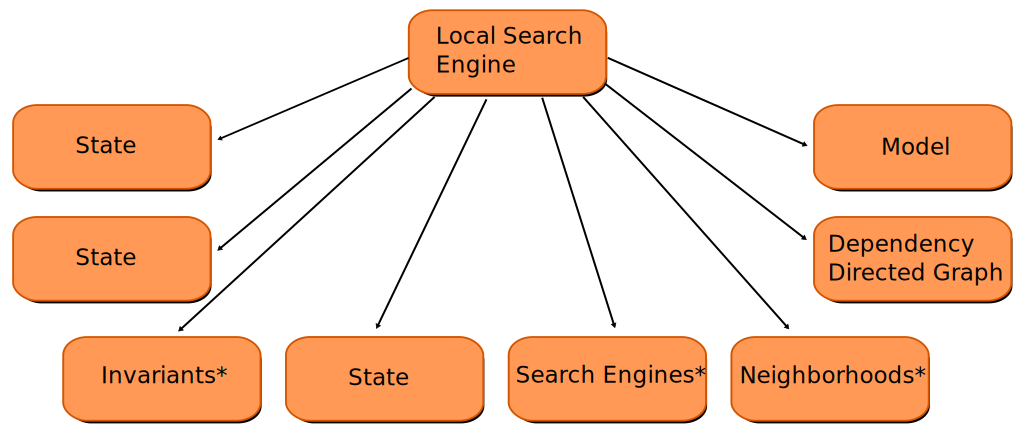
\includegraphics[width=0.9\linewidth]{LSE}\caption{Overview of the class pointers of \class{LocalSearchEngine}. The 
fields 
marked with a star (*) are several classes of that type.} 
\label{fig_lse}
\boste{Variable og constraint til venstre, think this should be posted earlier} 
\end{center}
\end{figure}\noindent




% For simplicity let us first consider the neighborhood operation involving changing the value 
% of a single 
% variable $x$. The change of variable value is send through the dependency digraph where each invariants, reachable from 
% the vertex representing $x$, is updated. The propagation queue is used to determine the sequence the invariants should 
% be updated. This will update invariants that represent violation of constraints with different priority and the 
% evaluation function. \\
% If a neighborhood operation consist of more variables changing values, such as swapping values of two variables, the 
% propagation queues 
% of these variables can be merged. The merging should remove duplicates and keep the invariants topological sorted. The 
% invariants unique time stamp can be used to keep the ordering. The new queue gives an ordering the invariants should be 
% updated such that they are only updated once during each neighborhood operation. \\ 
  \subsection{Neighborhoods}
  The neighborhood classes are all subclasses of the super class \class{Neighborhood} such that they can easily be 
combined with the search procedures. The methods of neighborhoods are illustrated in figure \ref{fig_neighborhood}.\\
\begin{figure}[t]
\centering
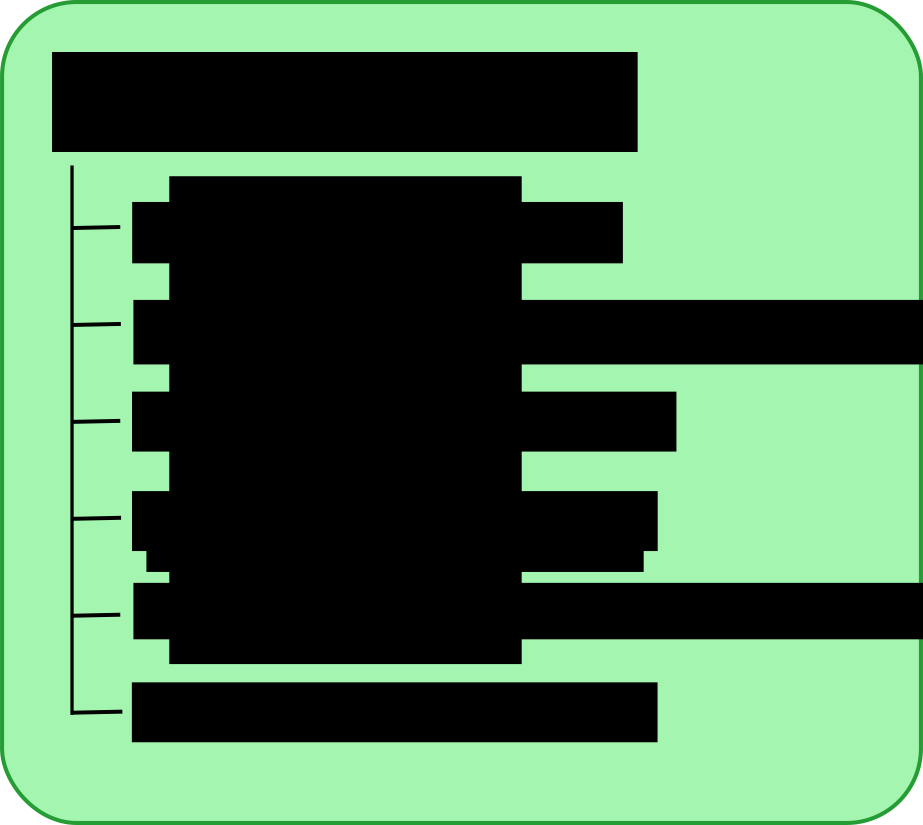
\includegraphics[width=0.9\linewidth]{neighborhood}
\caption{The methods all Neighborhood classes needs to implement.} 
\label{fig_neighborhood}
\end{figure} \noindent \noindent
All \class{Neighborhoods} implemented use a step function that changes value of a single independent variable, from 
0 to 1 or vise versa since all variables are binary. A neighborhood operation is stored in an a \class{Move} object 
that 
contains a pointer to the variable used, the variables change in value, and the change to the quality vector $Q$, 
once computed. The change in the quality vector is referred to at the \emph{delta vector}. \\ 
The \class{Neighborhood} classes that are implemented are shown in table \ref{tab_neighb}. \\  
\begin{table}[b]
\centering
\begin{tabular}{|l|l|}
\hline
class                          & Heuristic                                          \\ \hline
\class{FlipNeighborhood}     & All variables                                      \\ \hline
\class{RestrictedFlipNE}     & An expected 5000 variables chosen at random              \\ \hline
\class{ConflictOnlyNE}       & All variables in unsatisfied constraints           \\ \hline
\class{RandomConflictFlipNE} & Variables from a random unsatisfied constraint \\ \hline
\end{tabular}
\caption{Table of \class{Neighborhood} classes.}
\label{tab_neighb}
\end{table} \noindent
The method \method{next()} creates new \class{Move} object and returns a pointer to it. If all possible neighborhood 
operation of the neighborhood function have been returned the method returns a pointer to \textbf{NULL} instead. To know 
when  a neighborhood has been fully explored, counters and iterators are used depending on the neighborhood. These are 
reseted when returning \textbf{NULL} or the method \method{commitMove(move)} is called. The \class{Move} created only 
contain the variable and its suggested change in value, the delta vector is not computed yet. \\ 
For \class{FlipNeighborhood} when \method{next()} returns a \class{Move} and the variable chosen is given by a random 
sequence, a mask.  When \method{next()} is called in the \class{RestrictedFlipNE} class it returns the next variable 
probability $p = \frac{5000}{n}$, where $n$ is the number of independent variables. This gives expected 5000 variable 
before it return a \textbf{NULL} pointer. \\
For \class{ConflictOnlyNE} the neighborhood operations consist of a variable that participate in a constraint that is 
unsatisfied. \\ 
The class \class{RandomConflictFlipNE} chooses an unsatisfied constraint at random and returns a \class{Move} with 
a variable participating in that constraint until each \class{Move} with a different variable has been returned. \\
Method \method{nextRandom()} returns a \class{Move} with a random variable from the neighborhood.  \\ 
Method \method{calculateDelta(move)} takes a \class{Move} pointer as argument and propagate the change through the 
dependency digraph using the propagation queue of the variable. The method is identical for all the 
\class{Neighborhood} classes implemented. The method returns a flag that indicates if the suggested 
neighborhood operation is forbid by a oneway constraint. \\ 
The following describes how calculating the delta change of a variable $x_i$ changing value. 
\begin{enumerate} 
 \item Reset delta value of invariants in quality vector $Q$
 \item Send delta value of $x_i$ to neighbor invariants in DDG.
 \item For each invariant $y_j$ in propagation queue of $x_i$, calculate delta value $y_j$, if it is not zero, send 
the change to neighbors in DDG. 
 \item If a variables delta value is not allowed, by a oneway constraint, reset all delta values of invariant in 
the propagation queue. Then return false. 
 \item Otherwise update delta quality vector of move. 
\item return true if the $move$ is an allowed neighborhood operation. 
\end{enumerate} \noindent
The delta values of the invariants can be reset by calling \method{calculateDelta}, when no change is send. The 
reason for resetting them is only to make sure their stack of changes are empty before the next neighborhood operation 
is calculated. \\ 
To commit a neighborhood operation the method \method{commitMove(move)} is called with a pointer to the 
\class{Move} $move$ that is wanted. \method{commitMove(move)} recalculate the delta value 
by \method{calculateDelta(move)} since other neighborhood operation might have been explored since move was 
calculated last. Once the delta values of invariants have been computed, the invariants can be updated by calling their 
\method{updateValue()}. Invariants that represent violation of a single constraint are kept in a hash map of they are 
non zero. If they change value from non zero to zero or vise versa, that hash map needs to be updated. The hash map is 
used by the two neighborhoods \class{ConflictOnlyNE} and \class{RandomConflictFlipNE} that only can be used when the 
current solution is infeasible. If the current solution is feasible their neighborhood sizes are zero. \\
A default method \method{compareMoves(move1,move2)} compares the delta vector of two \class{Move} classes and 
returns 0 if they are the same, 1 if move1 is best and 2 otherwise. \\ 
The size of the neighborhood with the restriction applied to it, if any, can be requested from the 
method \method{getSize()}. It returns the size of the current neighborhood. For \class{ConflictOnlyNE} and 
\class{RandomConflictFlipNE} the neighborhood size can change after each iteration, for the others it is a constant 
size. \\ 


  \subsection{Search Procedures}
  \class{Neighborhood} classes do not implement any strategy of which neighborhood operation to choose. 
Search procedures are using a neighborhood and define this strategy. The classes implemented 
are \class{FirstImprovement}, \class{BestImprovement}, \class{TabuSearch}, and \class{RandomWalk}. \\
\class{FirstImprovement}, \class{BestImprovement}, and \class{RandomWalk} are implementation of local search 
algorithms of almost same name and can be used together with any of the \class{Neighborhood} classes. 
\class{TabuSearch} is an implementation of the metaheuristic tabu search using a tabu tenure, and 
an aspiration criteria. \medskip \\
The class \class{BestImprovement} looks at each \class{Move} a \class{Neighborhood} class $NE$ gives and finds the 
best \class{Move}. The best \class{Move} is determined from their delta vector after the method 
\method{calculateDelta()} of the \class{Neighborhood} is called on each \class{Move} returned by the neighborhood 
until \textbf{NULL} is returned. \class{BestImprovement} returns a boolean that tells if the current solution was 
improved. A boolean can be given to \class{BestImprovement} that indicate if it should commit a non improving 
\class{Move}. How each iteration is done is describe by algorithm \ref{algo_BI} \\ 
\IncMargin{1em}
\begin{algorithm}[H]

%\SetKwFunction{relation}{relation}\SetKwFunction{coeff}{coefficient}
\SetKwFunction{makeOneway}{makeOneway}
\SetKwFunction{defi}{defines}
\algdata
\Input{\bool alwaysCommit, \class{Neighborhood} NE}
\Output{\bool improvement}
\BlankLine
%\If{c \upshape already defines a oneway constraint}{\Return{} \false\; \boste{This constraint could be removed in 
%$O(\alpha(c_j))$}}
% \If{\upshape Number of integer variables not defined $> 1$}{\Return{} \false\; \boste{Needed in order to create the 
% right update queue}}
%\If{$|Y(c)| > 1$}{\Return{} \false}
%\If{\relation{c} \upshape is (==) }{\Return{} \true}
%\If{$c_j$ \upshape is not a linear equality}{
%  \Return{} \false}
%\int coeff = \coeff{c,v}\;
%\upshape in $\bigcup\limits_{o \in O} f_o(\vec{v})$}{	
%\tcp{Find the best variable to define}
\class{Move} bestMove = NE.next() \;
\class{Move} move = NE.next() \;
\While{move != NULL}{
  \bool allowed = NE.calculateDelta(move) \;
  \If{!allowed}{
    move = NE.next() \;
    \continue \;
  }
  bestMove = compareMove(move,bestMove) \;  
  move = NE.next() \;
}
\bool improvement = Check if bestMove gives improvement \;
\tcp{by looking at delta vector} \;
\If{improvement \textbf{OR} alwaysCommit}{
  NE.commitMove(bestMove)
 }
\Return improvement \;

\caption{BestImprovement Start} \label{algo_BI} 
 %\caption{Test if a constraint $c$ can define a variable $x$ } \label{algo_checkoneway}
\end{algorithm} \noindent
\DecMargin{1em} \\
If \class{BestImprovement} is combined with the neighborhood class \class{RandomConflictConNE} it gives a minimim 
conflict heuristic that can be useful to reach a feasible solution. \\ 
\class{FirstImprovement} has a very similar implementation. Instead of calculating each \class{Move} of a 
\class{Neighborhood} class $NE$ it stops requesting a \class{Move} once an improving \class{Move} is found. If no 
improving \class{Move} is found when $NE$ returns a \textbf{NULL} pointer it does not commit a \class{Move}. If no 
improving \class{Move} is found the current solution is in a local optima with the regard to the chosen 
\class{Neighborhood}. \\ 
The class \class{RandomWalk} uses the method \method{nextRandom()} from its \class{Neighborhood} $NE$ and if that 
\class{Move} is allowed it is committed. It takes an integer as argument that indicate the number of times it is 
repeated. The benefit is many iteration can be done but they are not as likely to have a good quality.  
Though tabu search is a metaheuristic it is implemented the same way as the other search procedures but with some 
additions. It takes four arguments; the number of iterations made so far, the best solution found, the current 
solution, and a tabu list. The implementation is similar to \class{BestImprovement} with additional checks with regard 
to the tabu list and aspiration criteria. The aspiration criteria is if a neighborhood operation is tabu but leads to a 
solution better than one found so far, the tabu list is ignored and that neighborhood operation is done. The 
tabu list has size $n$ and each variable has a integer corresponding to the last iteration that variable was 
changed. \\ 
The algorithm for tabu search for a single flip neighborhood sketched by algorithm \ref{algo_TS}. \\ 
\IncMargin{1em}
\begin{algorithm}[H]

%\SetKwFunction{relation}{relation}\SetKwFunction{coeff}{coefficient}
  \algdata
\Input{\int iteration, int[] best, int[] current, int[] tabulist }
%\Output{\bool improvement}
\BlankLine
\int tabuTenure = Random(0,10)+ min(NE.getSize()*2, tabulist.size() /200) \;
\class{Move} bestMove = NE.next() \;
\class{Move} move = NE.next() \;
\While{move != NULL}{
  \bool allowed = NE.calculateDelta(move) \;
  \If{!allowed}{
    move = NE.next() \;
    \continue \;
  }
  \bool isTabu = (iteration - tabulist[move.ID]) $<=$ tabutenure \;
  \If{isTabu}{
    \If{betterThanBest(current,move.getDeltaVector(), best)}{
      NE.commitMove(move)
      tabulist[move.ID] = iteration \;
      \Return \true \;
      
    }{
      move = NE.next() \;
      \continue \;
    }  
  }
  bestMove = compareMove(move,bestMove) \;  
  move = NE.next() \;
}
%\bool improvement = Check if bestMove gives improvement to current solution 
%\tcp{by looking at delta vector} \;
NE.commitMove(bestMove) \;
%\Return improvement \;

\caption{TabuSearch Start(iteration, best,current,tabulist)} \label{algo_TS} 
 %\caption{Test if a constraint $c$ can define a variable $x$ } \label{algo_checkoneway}
\end{algorithm} \noindent
\DecMargin{1em} \\
\class{TabuSearch} needs to be combined with a \class{Neighborhood} class that uses single flip neighborhood operation. 
This makes it less flexible in combining it with a \class{Neighborhood} class than the other search procedures 
\class{FirstImprovement}, \class{BestImprovement}, and \class{RandomWalk}. \\ 
In order to create an efficient local search we need to change search procedure at some point, with the exception of 
tabu search that can perform well on it own. 




\section{Tests}
\section{Results}
\section{Future Work}
  \boste{Short description of problems that should be investigated more} \\
\boste{preprocessing :} preprocessing of Cplex and gurobi with Gecode \\ 
\boste{Cycles :} Finding all (elementary) cycles in the dependency digraph and/or finding the smallest set of vertices 
to remove such that the graph is DAG. \\ 
\boste{Integer variables :} How to treat integer variables when they cannot be defined by oneway constraints. \\ 
\boste{Propagation queue :} Finding a datastructure better suited for propagation queues than red-black trees (C++ 
set). \\ 
\boste{Mixed neighborhood :} Find a way to treat both integer and binary variables in local search. \\
\boste{Make ``true'' DFS when creating propagation queues, no revisit of vertices} \\
\boste{Change Constraints to invariants during local search to measure the violation} 
\section{Conclusion}

\bibliographystyle{plain}
\bibliography{main}
%\newpage
%\newpage
%\section{Defenitions of structures in a solver}
%structure intro
%\subsection{variables}
%\subsection{Moves}
%\subsection{Constriants}
%\subsection{Invariant}
%\emph{Invariants} are variables, whose value are functionally defined by other variables. Invariants are introduced by 
the solver and neither the variable defined nor the variables defining the variable need not to be decision variables 
in the CSP or CSOP but can be auxiliary variables whose value are of interest. \\ 
\emph{One-way constraints} are constraints that defines the value of an invariant. 
\begin{equation}
 x = f(\mathbf{z}) 
\end{equation}
$f(\mathbf{z})$ is a \oneway with a set of input variables $z$ that functionally defines the \invar $x$. \\ \medskip



%currently in the system but they can be new auxiliary variables whose value are of interest. 
\iffalse
The invariants all have generic methods that needs to be defined for the different types of invariants. One of 
these 
methods is for instance \method{getCurrentValue()} that return the value of the invariant. If a variable $v$ 
changes value then the invariants that are defined by $v$ needs to update their current value. This is done 
through the \method{addChange(arguments)} method, \method{calculateDeltaValue()}, and  \method{updateValue()}. They 
informs the invariant something is changed, calculates the change in value and updates the current value respectively. 
Since invariants can be defined by variables that are invariants themselves this can leads to a series of 
updates. Invariants and constraints can built as a directed graph without cycles in 
order to avoid looking at an invariant multiple times when a change is made to a variable. The construction of that 
graph is described in section \ref{updategraph}. \\ 
An example of an invariant is the \method{Sum} invariant that defines an auxiliary variable. The 
\method{Sum} invariant consist of a coefficient set $C$, variable set $V$ and it can have a constant $b$ added. For 
a \method{Sum} invariant $S$ the value is defined as: \\
\begin{equation}
 S = b+ \sum_{\substack{i \in I_S}}  c_i x_i  
\end{equation}


One-way constraints are constraints that is used to define the value of a single variable. The single variable is made 
as an \class{invariant} and can only change when one of the variables that defines it changes. One-way 
constraints reduces the search space \boste{(which should be discussed before this I guess)} since the variable defined 
by a one-way constraint can only be changed by a move indirectly. 

\fi	

%which value is defined by the sum of the variables and invariant  times their coefficient. 
%Invariants are used to create auxiliary variables based on other variables and/or invariants. 
%\subsection{Oneway Constraints}
%One way constraints are constraints that is used to define a single variable. The single variable is made as an 
invariant and can only change when one of the variables or invariants that defines it changes. One way constraints 
reduces the search space (which should be descussed before this I guess) since the variable defined by a oneway 
constraint cannot be changed by a move. 
%\subsection{State}
%\subsection{Metaheuristics implemeted}
%\newpage
%\section{Existing Solvers}
%

\subsection{Comet}
% Figur om opbygning af comet som i bogen
Comet is an object orientated programming language that uses the modeling language of constraint programming and uses a 
general purpose local search solver. Comet is now an abandoned project but the architecture used is still of interest. 
The core of the language is the incremental store that contains various incremental objects fx. incremental variables. 
Invariants, also called one-way constraints, are expressions that are defined by incremental variables and a relation of 
those. An incremental variable $v$ can for instance be expressed as a sum of other variables. The variable $v$ will 
automatically be updated if one of the other variables changes value. The order in which the invariants gets updated can 
be implemented to achieve higher performance. \\ \medskip
One layer above the invariants is the differentiable objects that can use the invariants and the incremental objects. 
Both constraints and objective are implemented as differentiable objects. They are called differentiable 
because it is possible to compute how the change of a variable value will affect the differentiable object's values. 
All 
constraints are implemented using the same interface, that means that all constraint have some methods in common. These 
method is defined as invariants hence they are always updated when a change is made to one of their variables. This is 
especially useful when combining multiple constraints in a constraint system, that also implements the constraint 
interface. The constraints can be combined in a constraint system that then uses the method from the individual 
constraints to calculated its own methods. Just like the \interface{constraint} interface there exist a 
\interface{objective} interface. Both 
will be described further in section \ref{difObj}. \\ \medskip
The next layer is where the user models their problem and use the objects mentioned above. Several search method are 
implemented that can be used. The benefit of this architecture is the user can focus on modeling the problem 
efficiently on a high level and thereby avoid small implementation mistakes. Using constraint programming inspired 
structure gives the benefit of brief but very descriptive code.

\subsubsection{Invariants}



\subsubsection{Differentiable Objects} \label{difObj}
Comets core modeling object is the differentiable objects that are used to model constraints and objective functions. \\
All constraints in Comet implement the %\il{Constraint} interface (Hvad er et interface?) that makes it 
possible to combine the constraints and reuse them easily. A constraint has at least an array $a$ of 
variables as argument, that is the variables associated with the constraint. The interface specifies some basic 
methods that all constraints must implement such as \method{violations()} that returns the number 
of violations for that constraint and \method{isTrue()} that returns whether the constraint is satisfied. How the number 
of violations is calculated depends on the implementation of the constraint. An example could be the 
\method{alldifferent(a)} constraint, that states that all variables in the array $a$ should have distinct values. The 
method \method{violations()} then returns the number of variables that do not have a unique value. \medskip \\ 
% variables, value or decomposition based violations. Skal uddybes
One of the benefits that all constraints implements the same interface is the ease of combining these constraints. 
%%% Det her skal enten omskrives ingen logical combinators eller udlades.
This can be done by using other differentiable objects such as logical combinators. These objects has a specific 
definition of the basic methods from the \interface{Constraint} interface that means they do not rely on the semantics 
of the constraints to combine them. 
Another way to combine the constraints is to use a constraint system. Constraint systems are containers objects that 
contains any number of constraints. These constraints are linked by logical combinators, namely conjunction. Comet can 
use several constraints system simultaneously and is very useful for local search where one system can be used for hard 
constraints another for soft constraints. Other constraint operators in comet are cardinality constraints, weighted 
constraints and satisfactions constraints. \medskip \\
Objectives are another type of differentiable objects and the structure is very close to the structure of constraints. 
Objectives implements an interface \interface{Objective} that have some of the same methods as \interface{Constraint} 
but instead of having \method{isTrue()} and \method{violations()} they have \method{value()} and \method{evaluation()}. 
The method \method{value} returns the value of the objective but it can be more convenient to look at the method 
\method{evaluation()} to guide the search. The method \method{evaluation()} should indicate how close the current 
assignment of variables is to 
improve the value of the objective or be used to compare two assignments of variables. How the evaluation should do 
that depends on the nature of the problem and could for instance use a function that would decrease as the assignment 
of variables gets close to improve the \method{value()}.

%

%\subsection{Localsolver}
bla2 
%\input{OsCar}
%\newpage
%\section{Graph}
%There can be many dependencies between variables,invariants and constraints and these dependencies can be illustrated 
by a graph. The graph can be partioned into to parts. The first part consist of a vertex for each variable and two 
vertices $u$ and $v$ are connected if and only if they at least have one constraint in common. The edges can then be 
expressed as the constraints. The second partition of the graph consist of all the invariants. The  
  
%\newpage
%\subsection{Creating the Update Graph} \label{updategraph}
%Write the algorithm here
%\newpage
%\section{Structure (or Architecture?) of My Solver}
%\section{Tests}
%\section{Results}
%\section{Conclusion}

%The purpose of this solver is to combine the simplicity of constraint programming formulation with the 
efficiency local search. Constraint programming sometimes offers a natural way to write problem formulations that can 
lead to very short and precise formulation. Local search is effective at searching for an improvement of a current 
solution. \\ 
This solver is roughly split into three parts, one for formulating the problem, one for finding an initial solution and 
a part for improving the current solution. The user needs to define variables and constraints for the problem and 
give and need to specify an objective for optimization. The formulation given by the user is then parsed to a 
constraint programming solver Gecode and Local search framework. Gecode is used to find an initial solution that the 
local search framework will try to improve with regard to the objective given by the user.   

\subsection{Parsing the Problem Formulation}

\subsection{The User Surface}
\subsection{The Local Search}


% Generelle fejl

% Can, be precise -> is 
% Define 
% which og that 
% properly vs probably

\end{document}
